%%%%%%%%%%%%%%%%%%%%%%% file template.tex %%%%%%%%%%%%%%%%%%%%%%%%%
%
% This is a template file for P&S 
%
% Copy it to a new file with a new name and use it as the basis
% for your article
%
%%%%%%%%%%%%%%%%%%%%%%%%   EDP Sciences  %%%%%%%%%%%%%%%%%%%%%%%%%%
%
\documentclass{ps}
%
%%%%%%%%%%%%%--PREAMBLE--%%%%%%%%%%%%%%%%%%
%%-----------------------------
%%         ...........
%%         your macros
%%         ...........
%%-------------------------%%----
%\usepackage{epstopdf}% To incorporate .eps illustrations using PDFLaTeX, etc.
%\usepackage[caption=false]{subfig}% Support for small, `sub' figures and tables
\usepackage{multirow}

\usepackage[numbers,sort&compress]{natbib}% Citation support using natbib.sty
\bibpunct[, ]{[}{]}{,}{n}{,}{,}% Citation support using natbib.sty
\renewcommand\bibfont{\fontsize{10}{12}\selectfont}% Bibliography support using natbib.sty

\theoremstyle{plain}% Theorem-like structures provided by amsthm.sty
\newtheorem{theorem}{Theorem}[section]
\newtheorem{lemma}[theorem]{Lemma}
\newtheorem{corollary}[theorem]{Corollary}
\newtheorem{proposition}[theorem]{Proposition}

\theoremstyle{definition}
\newtheorem{definition}[theorem]{Definition}{\tiny }
\newtheorem{example}[theorem]{Example}

\theoremstyle{remark}
\newtheorem{remark}{Remark}
\newtheorem{notation}{Notation}
\usepackage[hidelinks]{hyperref}
\hypersetup{
	colorlinks   = true, %Colours links instead of ugly boxes
	urlcolor     = blue, %Colour for external hyperlinks
	linkcolor    = blue, %Colour of internal links
	citecolor   = red    %Colour of citations
}

\usepackage{xcolor}
\usepackage{graphicx}
\newcommand{\longeq}{\scalebox{4}[1]{=}}   %define wode equal sign

\usepackage{blindtext}
\usepackage{array}
\newcolumntype{R}{r@{}}
%%%%%%%%%%%%%%%--BODY--%%%%%%%%%%%%%%%%%%
\begin{document}
%%-----------------------------
%%      the top matter
%%-----------------------------
\title{A New Formulation of Generalized Gamma: Some Results and Applications} %\thanks{...}\thanks{...}% At most 5 thanks
%
\author{Cheng Peng}\address{Department of Mathematics, West Chester University, West Chester, PA, 19383 USA}
%\author{...}\address{...}
%\author{...}\address{...}
%
%\date{9/23/2023}
%
\begin{abstract}  
		We extend the 2-parameter Weibull to the generalized gamma distribution by adding a new partial parameter. The new shape parameter can be used to easily generate generalized gamma distributions with different shapes of the density function, hazard rate, and mean residual lifetimes that are useful in simulating various business processes such as manufacturing processes, and reliability systems. We derived some theoretical results and created visual presentations to show the influence (or effect) of this new shape parameter as well. A new Monte Carlo simulation based on the new parameter was proposed to assess the discrepancy between the generalized gamma and its subfamilies. The power analysis of the proposed test was evaluated via simulation studies. We also present some numerical examples.
\end{abstract}
%
%\begin{resume} ... \end{resume}
%
\subjclass{MSC2010: 62E10, 62E20, 62F05, 62F12, 62N02}
%
\keywords{Generalized gamma family;  survival and reliability analysis; Kullback-Leibler divergence; business and statistical simulations; Monte Carlo test.}
%
\maketitle
%%-----------------------------
%%      your text
%%-----------------------------
%\section*{Introduction and Related Work}
\section{Introduction and Related Work}
The standard two-parameter Weibull distribution has the following density   

\begin{equation}\label{Weibull-dist}
	f(x) = ab^{-a}x^{a-1}\exp[-(x/b)^a]
\end{equation}

\noindent where $a$, $b$, $x > 0$.  $a$ is the shape parameter and $b$ is the scale parameter. The Weibull distribution and its variants have been extensively studied and widely applied in quality engineering, reliability analysis, and survival modeling (in clinical studies). See monographs of Dodson \cite{Dodson-2006}, McCool \cite{McCool-2012}, Murthy et al \cite{ Murthy-Xie-Jiang-2004}, and Rine \cite{Rine-2008}. 


In reliability and clinical study, the hazard rates can have any pattern such as the work of Glaser \cite{Glaser-1980}  for bathtub hazard (BT),  Langlands et al  \cite{Langlands-Pocock-Kerr-Gore-1979} for the upside-down bathtub (UBT) hazard,  Bennette \cite{Bennette-1983} and Efron \cite{Efron-1988} and Gupta and Viles \cite{Gupta-Viles-2013}  roller-coaster hazard. However, the two-parameter Weibull can take only a monotonic failure rate across the entire lifetime limiting its applications to real-world problems. To obtain more flexible hazard rates, researchers have developed different ways to extend the Weibull to larger families. Some of the earlier work was due to Mudholkar et al \cite{Mudholkar-Srivastava-1993, Mudholkar-Srivastava-Freimer-1995, Mudholkar-Srivastava-Kollia-1996}. In the past decades, many such generalized Weibull distributions were proposed and studied. See, for example, Lai et al \cite{Lai-Xie-Murthy-2003},  Nadarajah and Kotz \cite{Nadarajah-Kotz-2005}, Bebbington \cite{Bebbington-Lai-Zitikis-2007},  Carrasco et al \cite{Carrasco-Ortega-Cordeiro-2008}, Pham and Lai \cite{Pham-Lai-2007}, Silva et. al \cite{Silva-Ortega-Cordeiro-2010},  Singla \cite{Singla-Jain-Sharma-2012},  Ortega et al \cite{Ortega-Cordeiro-Kattan-2013}, Xu and Peng \cite{Xu-Peng-2014} and Gauss et al \cite{Gauss-Cordeiro-Lima-Gomes-Silva-Ortega-2016}. In his monograph, Lai \cite{Lai-2013} systematically introduced various generalized Weibull distributions. Most recently, Almalki and Nadarajah \cite{Almalki-Nadarajah-2014} gave an up-to-date and comprehensive review of numerous extended Weibull distributions.


In this paper, we propose a new extension of the Weibull distribution by including an additive gamma shape parameter in the two-parameter Weibull density to obtain the well-known generalized gamma distribution (GG) after reparametrization. The generalized gamma was initially proposed by Stacy \cite{Stacy-1962} as an extension of the gamma distribution. Since the GG model has several well-known distributions as special cases and has flexible shapes of density and hazard rate, it has received wide attention from researchers and practitioners in both statistics and other relevant areas. See, for example, the work of Stacy and Mihram \cite{Stacy-Mihram-1965}, Harter \cite{Harter-1967}, Lawless \cite{Lawless-1980},  Diebold and Rudebusch \cite{Diebold-Rudebusch-1990}, Pham and Almhana \cite{Pham-Almhana-1995}, Allenby et al. \cite{Allenby-Leone-Jen-1999}, Dadpay et al. \cite{Dadpay-Soofi-Soyer-2007}, Gomes et al. \cite{Gomes-Combes-Dussauchoy-2008}, Kaniovski and Peneder \cite{Kaniovski-Peneder-2008}, Noufaily and Jones \cite{Noufaily-Jones-2013a, Noufaily-Jones-2013b} and Balakrishnan and Pal \cite{Balakrishnan-Pal-2015}. 


The focus of this paper is two-fold. The first objective is to study the geometric properties of the new parameter to see how it affects the shape of density, hazard rate, and mean residual lifetime functions. These properties are practically important in simulating various business processes (usually in the stage of the "what-if analysis" stage) for better business planning. The second objective is to develop a Monte Carlo simulation-based goodness-of-fit test to assess the departure from its subfamilies. It will be used together with other large sample tests in the data analysis to avoid misspecification (under or overfitting the data to a member of this family).


The rest of this paper is organized as follows. In Section \ref{sec02: model-formulation}, we outline the new formulation of the GG model from the Weibull distribution.  Some characterizations on the shape of density, failure rate, and mean residual lifetime functions are presented in Sections \ref{sec03:pdf-shape} and \ref{sec04:hazard-rate}. The information-theoretic analysis on the discrepancy between the generalized gamma and the Weibull using Kullback-Leibler divergence (KLD) is presented in Section \ref{sec05:information-analysis}. Maximum likelihood estimation of the parameter is developed in Section \ref{sec06:MLE}. In Section \ref{sec07:asymp-tests}, we present a novel Monte Carlo simulation-based goodness-of-fit test. A simulation study on the power of the novel Monte Carlo test is given in Section \ref{sec08:Simulation}. Several numerical examples from the generalized family with different applications are discussed in Section \ref{sec09:Numerical-examples}.  Some discussions are given in the concluding Section \ref{sec10:conclusion}. Finally, some proofs are given in the appendix. 




\section{Extending Weibull to Generalized Gamma } \label{sec02: model-formulation}

We add a gamma shape parameter $c$ and an adjusted normalizing coefficient to the standard two-parameter Weibull density to get the following new formulation of the generalized gamma density function
\begin{equation}\label{new-GG-pdf}
	g(x)=\frac{ab^{-a-c}x^{a+c-1}\exp[-(x/b)^a]}{\Gamma[(a+c)/a]}
\end{equation}
\noindent where $c$ is the added new partial shape parameter that satisfies $c+a > 0$. As usual, $a > 0$ and $b > 0$ are shape and scale parameters respectively. $a$ is the shape parameter that is analogous to the shape parameter in the regular Weibull distribution. If $a = 1$, the GG is reduced to the regular gamma distribution and $c+1$ is the gamma shape parameter. In other words, $c$ controls the shape of the reduced gamma distribution. For convenience, we will hereafter call $a$ and $c$ the Weibull and gamma shape parameters respectively.


\subsection{Visual Inspection of Shape Parameters}\label{visualizing-shape-parameters}


The shape of a density curve plays an important role in real-world applications in process capability index analysis. The above newly formulated GG density function has two shape parameters $a$ and $c$. As a visual exploration, we look at how the two shape parameters behave with the fixed scale parameter $b = 1$. We will do more analysis on the shape of the above density in the next section.   



\begin{figure}[h!]
	\centering 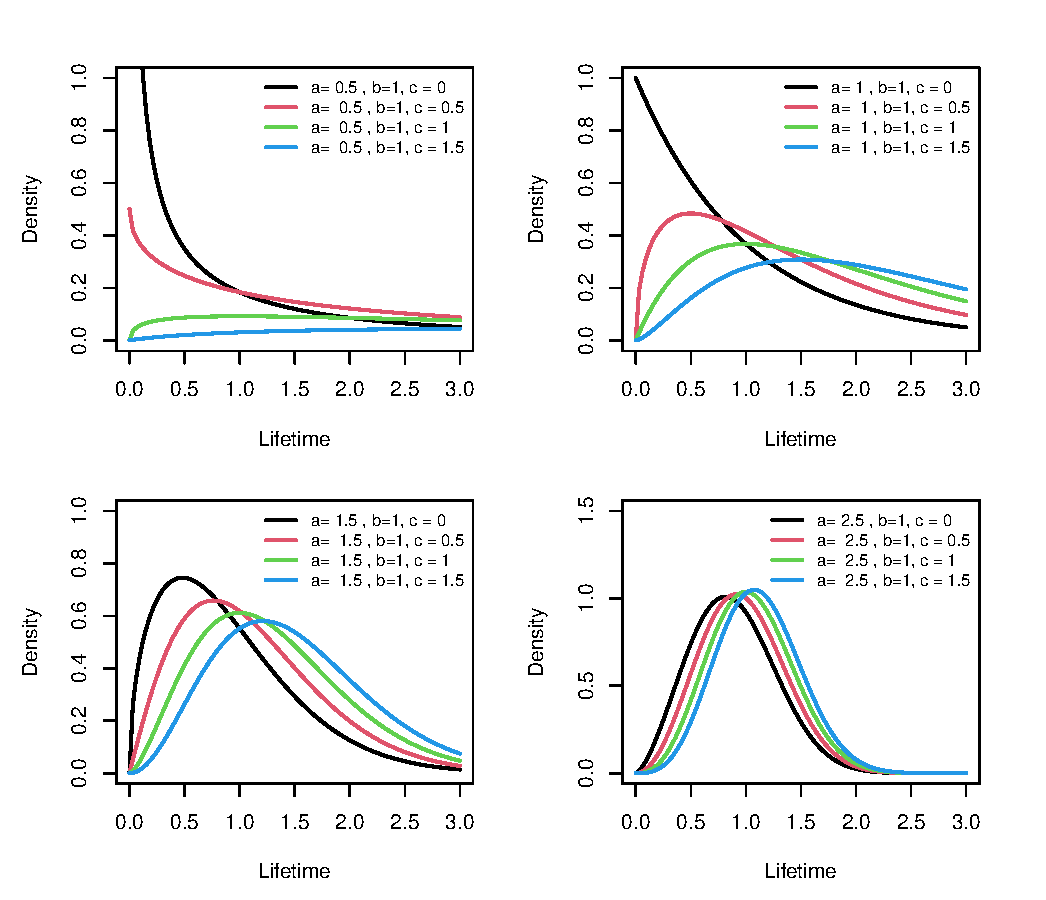
\includegraphics[width=10cm,height=9cm]{Figure01_pos_c_val.eps}
	\caption{The solid curve in each panel represents the standard two-parameter Weibull density. The scale parameter is chosen to be 1 in all panels. The values of the gamma shape parameter c in the extended Weibull distributions are all positive.}
	\label{fig01:Figure01_pos_c.eps}
\end{figure}

We can see from each plot in Figure \ref{fig01:Figure01_pos_c.eps} that, for the fixed value of $a$, the right tail of the density curves becomes heavier as the gamma shape parameter $c$ gets bigger. However, for a fixed value of the shape parameter $c$, we see across the plots and find that the right tail of the density curve gets lighter as the shape parameter $a$ increases. 

\begin{figure}[h!]
	\centering	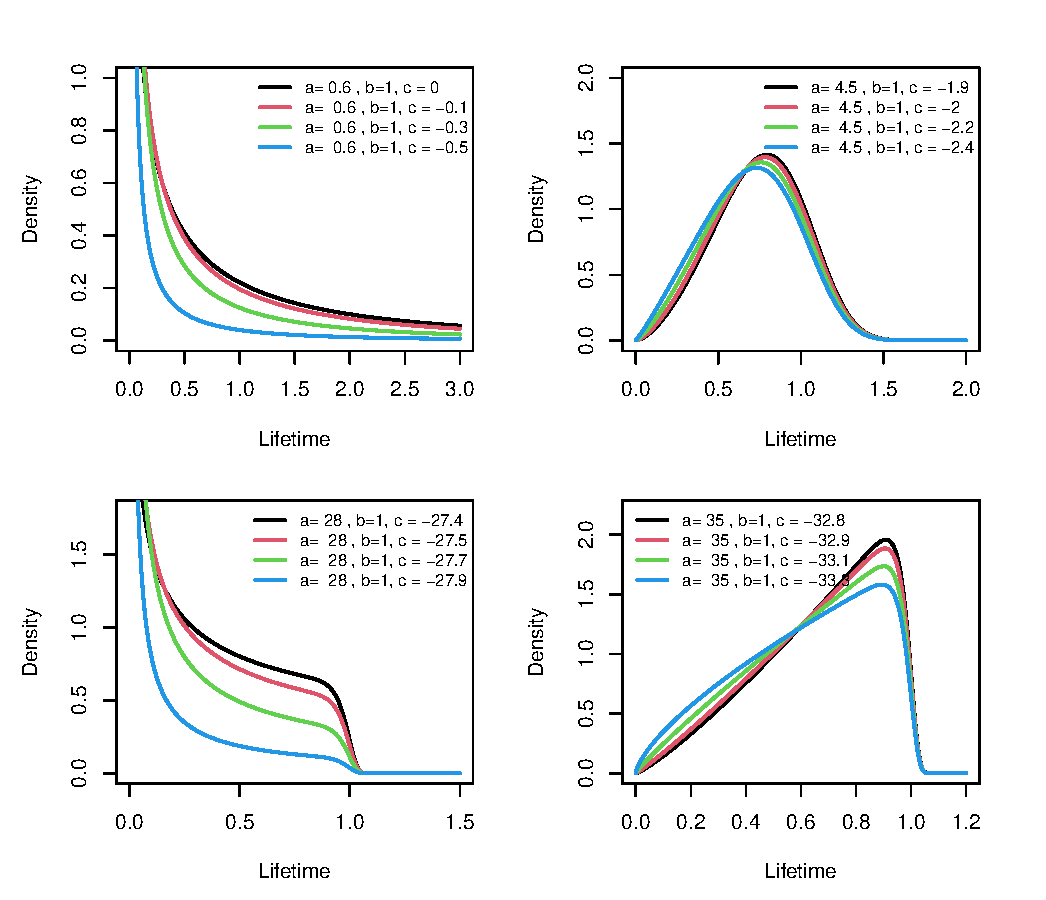
\includegraphics[width=10cm,height=9cm]{Figure02_neg_c_val.eps}
	\caption{The solid curve in each panel represents the standard two-parameter Weibull density. The scale parameter is chosen to be 1 in all panels. The values of the partial shape parameter c in the extended Weibull distributions are all negative. }
	\label{fig02:Figure02_neg_c.eps}
\end{figure}

Note that all values of $c$ in Figure \ref{fig01:Figure01_pos_c.eps} are non-negative.  In Figure \ref{fig02:Figure02_neg_c.eps}, we choose different sequences of negative values for the new partial shape parameter $c$  and a sequence of positive values of shape parameter $a$. We observe the sample pattern as we saw in Figure \ref{fig01:Figure01_pos_c.eps}. 


The exploratory visual analysis indicates that the two shape parameters behave in opposite ways. The bigger the value of the partial shape parameter $c$, the longer the right tail of the density for the fixed shape parameter $a$. However, for the fixed $c$, the bigger the value of $a$, the longer the left tail of the density.  



\subsection{Quantile Function and Moments} 

The cumulative probability distribution of the newly formulated GG (we will simply call GG hereafter) is given by
\begin{equation}\label{new-GG-CDF}
	F_{GG}(x)=\int_0^x\frac{ab^{-a-c}t^{a+c-1}\exp[-(t/b)^a]}{\Gamma[(a+c)/a]}dt = \frac{\gamma \left[(a+c)/a, (x/b)^a \right]}{\Gamma[(a+c)/a]}
\end{equation}
\noindent where
\begin{equation}
	\gamma \left[(a+c)/a, (x/b)^a \right] = \int_0^{(x/b)^a}y^{c/a}\exp(-y)dy
\end{equation}
\noindent is the lower incomplete gamma function. 

Note that we can re-express the CDF of the generalized gamma distribution as
\begin{equation}
	F_{GG}(x) = \frac{\gamma \left[(a+c)/a, (x/b)^a \right]}{\Gamma[(a+c)/a]} =\int_0^{(x/b)^a}\frac{y^{(a+c)/a-1}\exp(-y)}{\Gamma[(a+c)/a]}dy = G_0\left( [x/b]^a \right),
\end{equation}

\noindent where $G_0(y)$ is a special Gamma distribution with shape parameter $(a+c)/a$ and scale parameter to be unity. The density of this special gamma distribution is given by
\begin{equation}\label{special-gamma-dist}
	g_0(y) = \frac{y^{[(a+c)/a]-1}\exp(-y)}{\Gamma[(a+c)/a]}, y > 0.
\end{equation}

Using the inverse of the composite function, we can find the quantile function
\begin{equation}\label{quantile-fun}
	F_{GG}^{-1}(q:a,b,c) = b\left[ G_0^{-1}(q) \right]^{1/a}
\end{equation}
\noindent where $ G_0^{-1}(q)$ is the quantile function of $G_0(x)$ with shape $(a+c)/a$ and unity scale.

We will use the above relationship to generate random numbers for the GG using the existing computer programs for regular gamma CDF in the simulation study. To be more specific, if $U$ is a uniform random variable on $(0,1)$, then $X =  b\left[ G_0^{-1}(U) \right]^{1/a}$ has the distribution $F_{GG}(x)$.


We see from subsection \ref{visualizing-shape-parameters} that the shape of the GG density is very flexible, we can use the above quantile function to solve real-world application problems such as capability analysis of skew processes that involve quantiles. 



The k-th moment is given by
\begin{equation}\label{k-th-moment}
	\mu^k = E[X^k] = \int_0^\infty \frac{x^kab^{-a-c}x^{a+c-1}\exp[-(x/b)^a]}{\Gamma[(a+c)/a]}dx = \frac{b^k\Gamma[(a+c+k)/a]}{\Gamma[(a+c)/a]}.
\end{equation}

Some moment properties will be used in both characterizations and inference in the subsequent sections.


\section{Characterizations on  Density Shape}\label{sec03:pdf-shape}


The shape of the density function plays an important role in many practical applications such as process capability analysis (in environmental process control and manufacturing/production process monitoring) in which capability measures are customarily defined based on the shape of the probability density function of the underlying process.


\subsection{General Moments of Generalized Gamma}\label{sec3.1: preliminary-Digamma}


We first present several functions defined based on the gamma function. The digamma function (also called Euler $\Psi$ function) is defined to be


\begin{equation}\label{digamma-fun}
	\Psi(x) = \frac{d \ln\Gamma(x)}{dx} = \frac{\Gamma^\prime (x)}{\Gamma(x)}
\end{equation}
\noindent where
$$
\Gamma(x) = \int_0^\infty t^{x-1}e^{-t}dt.
$$
There are several different representations of the digamma function. We use the following integral representation given in Proposition 2.12 of Medina and Moll \cite{Medina-Moll-2009}.
$$
\Psi(\alpha) = \int_0^\infty \left[\frac{e^{-x}}{x}-\frac{e^{-\alpha x}}{1-e^{-x}} \right]dx.
$$
The high-order derivatives of the digamma function are called polygamma functions. These special functions are useful in characterizing the behavior of the partial parameter c in this paper. The integral and series representations of the polyganma functions are given by
$$
\Psi_n(\alpha)=\frac{d^n\Psi(\alpha)}{d\alpha^n} = \frac{d^{n+1}\ln \Gamma(\alpha)}{d\alpha^{n+1}} 
$$
\begin{equation}\label{polygamma-fun}
	= (-1)^{n+1}\int_0^\infty \frac{x^n e^{-\alpha x}}{1-e^{-x}}dx = (-1)^{n+1}n!\sum_{k=0}^\infty \frac{1}{(k+\alpha)^{n+1}}
\end{equation}

\noindent for $a > 0$ and any number n. See eq. 5.5 of Alzer \cite{Alzer-1997}. $\Gamma_1(\alpha)$ and $\Psi_2(\alpha)$ are called trigamma and tetragamma functions respectively.

\begin{figure}[h!]
	\centering	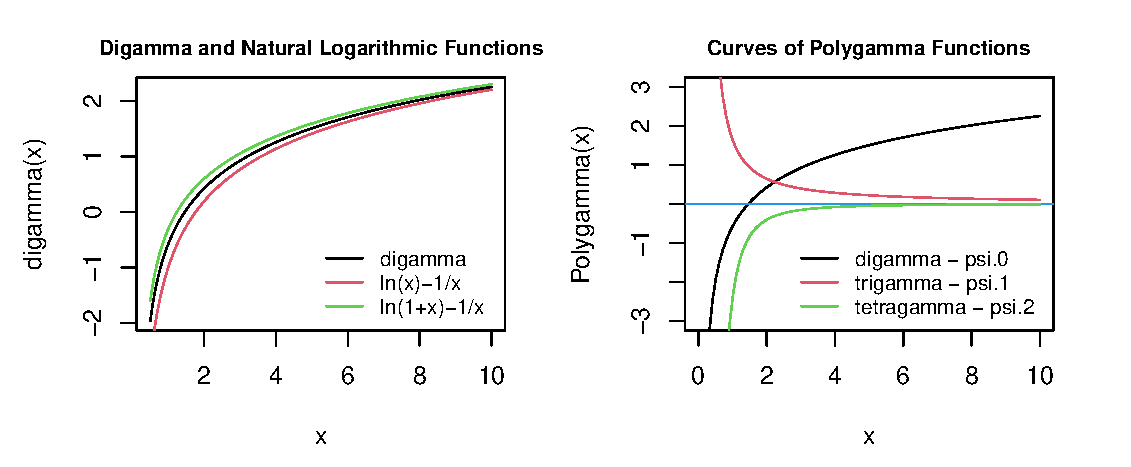
\includegraphics[width=12cm,height=5cm]{Figure03_Digamma_curves.eps}
	\caption{\emph{Left panel}: Bounds of digamma function. Since both bounding functions are monotonically increasing and have the same range from negative infinity to positive infinity, the digamma function is also monotonically increasing from negative infinity to positive infinity. \emph{Right Panel}: The trigamma is a decreasing positive function on $[0, \infty)$ while the tetragamma is an increasing negative function $[0, \infty)$.}
	\label{Fig03:Digamma_curves}
\end{figure}

\begin{lemma}\label{lemma3.1}
	Assume $x > 0$, following monotonic properties of polygamma functions hold.\\
	(a). Digamma $\Psi(\alpha)$ is increasing in $\alpha$.\\
	(b). Trigamma $\Psi_1(x) > 0$ and is decreasing.\\
	(c). Tetragamma $\Psi_2(x) < 0$ and is increasing.
\end{lemma}

\begin{proof}
	(b) and (c) are obvious from the series representation. The proof of (a) is trivial since in trigamma function $\Psi_1(x)$  is positive. 
\end{proof}

The next result describes the relationship between the digamma and the natural logarithmic function. This also implies that the range of the digamma function is $(-\infty, \infty)$.

\begin{lemma}\label{lemma3.2}
	Bounds of polygamma functions. For all positive x, we have \\
	(a). $\ln(x)-1/x < \Psi(x) < \ln(x+1) - 1/x$.\\
	(b). $\frac{(n-1)!}{x^n}+\frac{n!}{2x^{n+1}} < (-1)^{n+1}\Psi_n(x) < \frac{(n-1)!}{x^n}+\frac{n!}{x^{n+1}}$.
\end{lemma}

\begin{proof}
	(a)  see Corollary 2.3 of Muqattash and Yahdi \cite{Muqattash-Yahdi-2006}.\\
	(b)  see Lemma 1 of Guo and Feng \cite{Guo-Feng-2013}.  
\end{proof}

The following integrals due to Gradshteyn and Ryzhik \cite{Gradshteyn-Ryzhik-2007} are related to the digamma function. These integrals will be used to prove results regarding some general moments.

\begin{lemma}\label{lemma3.3}
	For positive $\nu$ and $\mu$ , we have the following integrals
	$$ (a). \hspace{3mm}\int_0^\infty x^{\nu-1}e^{-\mu x} \ln(x) dx = \mu^{-\nu}\Gamma(\nu)\left[\Psi(\nu) - \ln(\mu)\right]\hspace{25mm}$$
	$$ (b). \hspace{3mm}\int_0^\infty x^{\nu-1}e^{-\mu x} \left[\ln(x)\right]^2 dx = \mu^{-\nu}\Gamma(\nu)\left\{ \left[ \Psi(\nu) - \ln(\mu) \right]^2 +\Psi_1(\nu) \right\}$$ 
	where $\Psi(z)$  and $\Psi_1(z)$  are digamma function and trigamma function respectively. 
\end{lemma}

The following general moments based on the generalized gamma (GG) models will also be used in the subsequent discussions.

\begin{lemma}\label{lemma3.4}
	Let $X$ be the shape-modified Weibull distribution (GG) with parameters $(a, b, c)$ given before. The expectation of $(X/b)^k\ln(X/b)$ and $(X/b)^k\ln^2(X/b)$ are given respectively by 
	$$\mbox{(a)}. \hspace{3mm}E_{GG}\left[\left(X/b\right)^k \ln(X/b)\right] = \Gamma[(p+k)/a]\Psi[(p+k)/a]/\left\{ a\Gamma(p/a)\right\}\hspace{10mm}  \ \ \ \ \ \ \ 
	$$
	$$\mbox{(b)}. \hspace{3mm}E_{GG}\left[\left(X/b\right)^k \left[\ln(X/b)\right]^2\right] = \frac{\Gamma[(p+k)/a]\left\{\Psi^2[(p+k)/a] +\Psi_1[(p+k)/a]\right\}}{ a^2\Gamma(p/a)}$$
	where k is a positive real number and $p = a + c$. 
\end{lemma}

\begin{proof}
	See the proof in the appendix. 
\end{proof}

\subsection{Analysis of Density Shape}\label{subsec:density-shape}

Before presenting the main result on the shape of the density curve, we prove the following lemma describing the mode of the GG distribution. 

\begin{lemma}\label{lemma3.5}
	Assuming the parametrization of the GG model (\ref{new-GG-pdf}), we have the following results\\
	(a). If $a + c \le 1$, the GG has no mode.\\
	(b). If $a + c > 1$, the GG has a single mode.
\end{lemma}

\begin{proof}
	Taking the derivative of the logarithmic density function concerning x and setting it to zero, we have
	$$
	\frac{d}{dx}\ln g(x) = \frac{a+c-1}{x}-a\left( \frac{x}{b}\right)^{a-1}=\frac{(a+c-1)b^{a-1}-ax^a}{xb^{a-1}}=0
	$$
	If $a+c<1$, then $d\ln g(x)/dx < 0$ meaning that the GG density function is monotonically decreasing. This implies that the GG distribution has no mode. If $a + c > 1$, the above equation has a unique solution
	$$
	x = b\left( \frac{a+c-1}{ab} \right)^{1/a}.
	$$
	This implies that the GG is a unimodal distribution. 
\end{proof}

The following theorem characterizes how the gamma shape parameter affects the tail behavior of the GG distribution.

\begin{theorem}\label{thm3.1}
	Assuming the parameterization of the generalized gamma density in (\ref{new-GG-pdf}), we define a function of the gamma shape parameter c based on the generalized gamma density function as follows
	$$
	g_0(c)=\frac{ab^{-a-c}x^{a+c-1}\exp[-(x/b)^a]}{\Gamma[(a+c)/a]}
	$$	
	\noindent where $a$, $b$, and $x$ are considered as constant scalars. Then, for any given positive triple $(a, b, x)$, there exists a unique $c_0$, such that $g_0^\prime(c)>0$ for $-a < c < c_0$  and $g_0^\prime(c) < 0$ for $c > c_0$.
\end{theorem}

\begin{proof}
	Since $g_0(c)$ and $\ln g_0(c)$ have the same monotonic intervals. We proceed to examine the monotonicity of $\ln g_0(c)$. Note that
	$$
	\ln g_0(c) = \ln(a) - (a-c)\ln (b) + (a+c-1)\ln (x) - (x/b)^a - \ln \Gamma[(a+c)/a].
	$$	
	The partial derivative with respect to c is given by
	$$
	\frac{d}{dc}\ln g_0(c)=\ln\left( \frac{x}{b} \right)-\frac{\Psi[(a+c)/a]}{a}.
	$$
	By Lemmas \ref{lemma3.1} and \ref{lemma3.2}, $\Psi[(a+c)/a]$ is increasing in $(a+c)/a$. Hence, $\Psi[(a+c)/a]$ as a function of $c$ is increasing in $c$. This implies that $d g_0(c)/dc$  is a decreasing function of $c$ with domain $ a < c < +\infty$ and range $-\infty < c < +\infty$.  Consequently, there exists a unique $c_0$ such that 
	$$
	\frac{d}{dc}\ln g_0(c) > 0 \mbox{   for   } -a < c < c_0  \mbox{        and        } 
	%$$
	%\noindent and
	%$$
	\frac{d}{dc}\ln g_0(c) < 0 \mbox{   for   }   c > c_0
	$$
	Therefore, $g_0^\prime(c) > 0 $ for $-a < c < c_0$ and $g_0^\prime(c) < 0 $  for $c > c_0$.  The proof is complete.  
\end{proof}

The geometric implication of Theorem \ref{thm3.1} is straightforward: for fixed $a$, $b$ and $x$, we solve for $c_0$ from the following nonlinear equation
$$
\ln\left( \frac{x}{b}\right) -\frac{\Psi[(a+c)/a]}{a} = 0
$$

If  $-a < c < c_0$, as $c$ increases, the GG density $g(x)$ increases in $c$. In other words, increasing the value of c on the left of $c_0$ lifts the density curve upwards which makes the left tail of the density thicker. However, if $c > c_0$, as $c$ increases, the GG density $g(x)$ decreases in $c$. This means increasing the value of $c$ on the right of $c_0$ pulls the density curve upwards which makes the right tail of the density curve thinner.  


As mentioned earlier, the shape of the density curve is important in modeling process capability in statistical quality control. Specific applications of the GG model in process capability analysis and quality selection will be addressed separately elsewhere.


\section{Reliability and Survival Analysis}\label{sec04:hazard-rate}


This section discusses the reliability properties of the proposed GG distribution. We focus on the analysis of the hazard rate function. Note that the survival function of the GG distribution is given by


\subsection{Hazard Rates Function}\label{HR}


The bathtub and upside-down bathtub hazard rates are common in reliability and production engineering. Many consumers' product life cycles strongly exhibit the bathtub curve. Identifying turning points of a hazard rate function is critically important in reliability analysis. 



\begin{equation}\label{survival-fun}
	S_{GG}(x) = \int_x^\infty \frac{ab^{-a-c}t^{a+c-1}\exp[-(t/b)^a]}{\Gamma[(a+c)/a]}dt=\frac{\Gamma[(a+c)/a, (x/b)^a]}{\Gamma[(a+c)/a]}.
\end{equation}

The hazard rate function is then given by

\begin{equation}\label{hazard-rate}
	h(x) = \frac{ab^{-a-c}x^{a+c-1}\exp[-(x/b)^a]}{\Gamma[(a+c)/a, (x/b)^a]}
\end{equation}
\noindent where
$$
\Gamma[(a+c)/a, (x/b)^a]=\int_{(x/b)^a}^\infty y^{c/a}\exp(-y) dy
$$
is the upper incomplete gamma function. 

The shape of the hazard rate function is depicted in the following Figures \ref{Figure04_pos_c_hr} and \ref{Figure05_neg_c_hr}.

\begin{figure}[h!]
	\centering	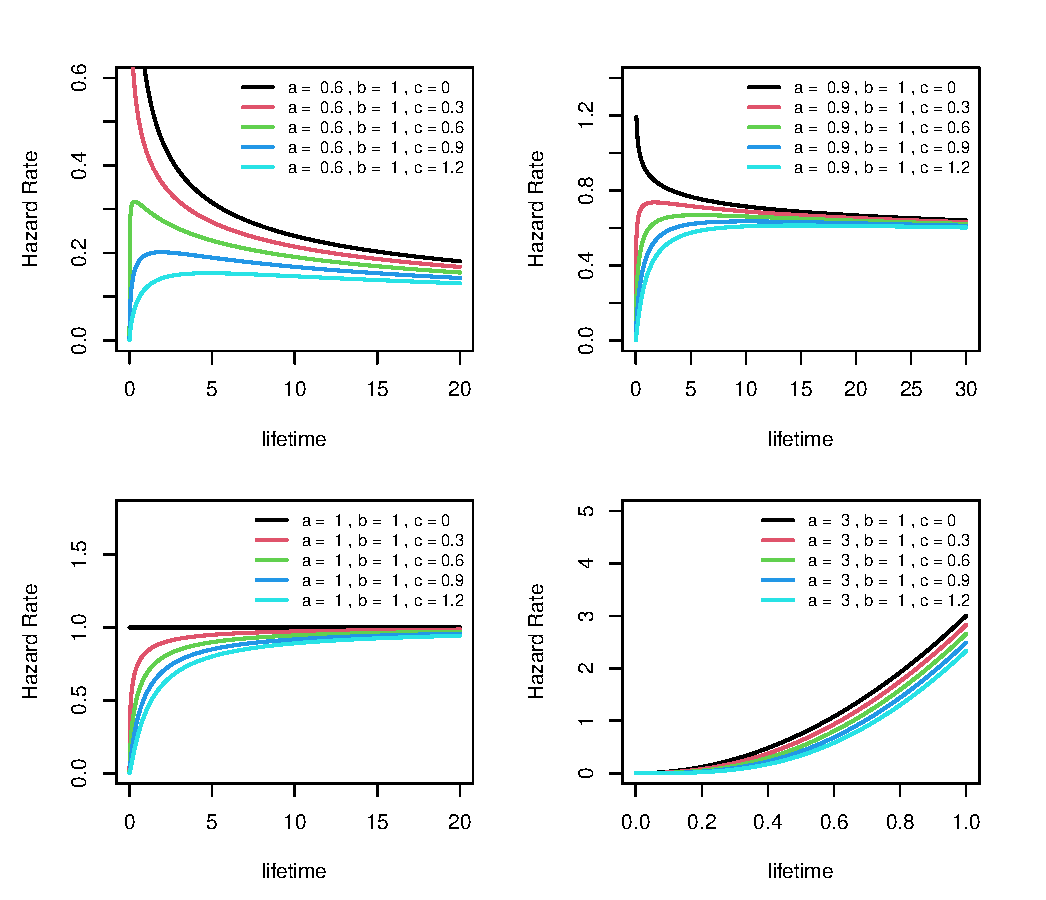
\includegraphics[width=10cm,height=10cm]{Figure04_pos_c_hr.eps}
	\caption{Adding the gamma shape parameter c changes the monotonicity of the hazard rate function. The solid curve is the hazard rate based on the standard two-parameter Weibull distribution. The top two panels contain some upside-down bathtub (UBT) hazard rates.}
	\label{Figure04_pos_c_hr}
\end{figure}

We can see from Figure \ref{Figure04_pos_c_hr} that the hazard rate of the GG model is always smaller than that of the standard Weibull model when $c > 0$. Note that the gamma shape parameter can take on negative values that satisfy $a + c > 0$. This choice of a negative value for the gamma shape parameter could result in a bathtub shape hazard rate (see Figure \ref{Figure05_neg_c_hr}). The hazard rate of the GG model is always bigger than that of the standard Weibull model when $c < 0$.


\begin{figure}[h]
	\centering	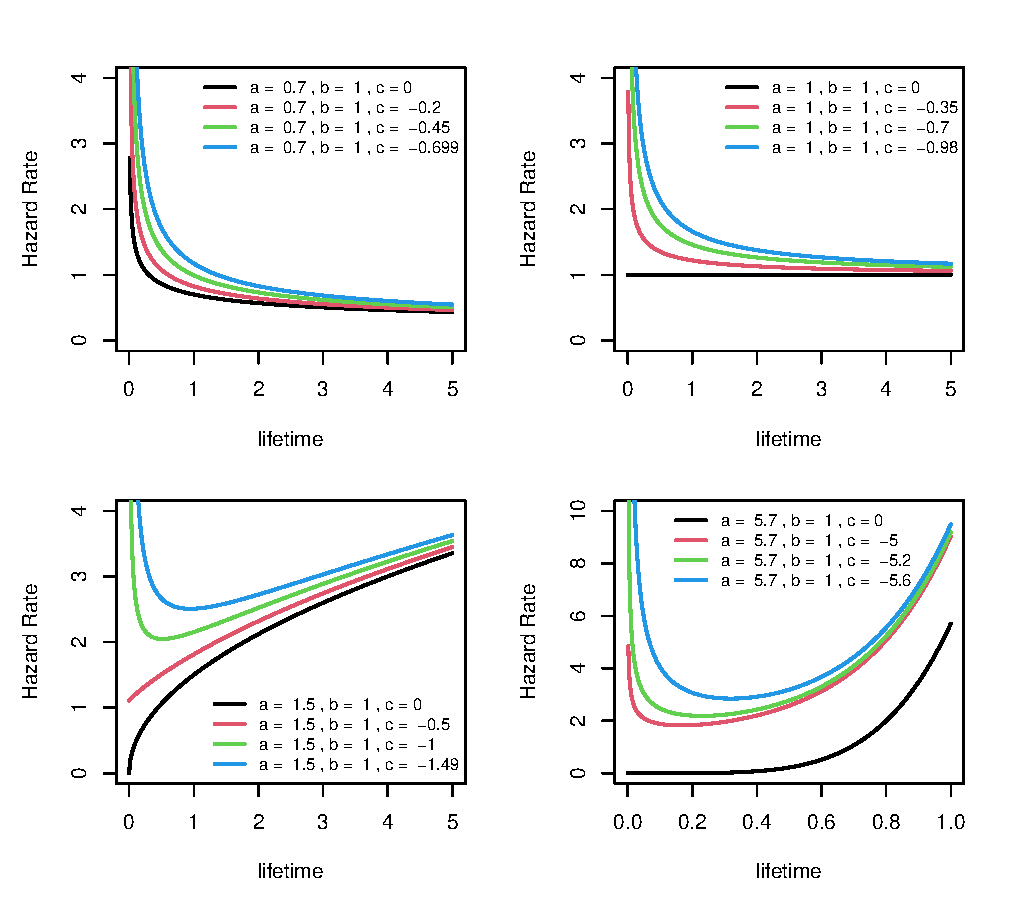
\includegraphics[width=10cm,height=10cm]{Figure05_neg_c_hr.eps}
	\caption{The hazard rate curve of the proposed GG model is based on the choice of the negative gamma shape parameter. All hazard curves in the bottom two panels are bathtub-shaped except the one based on the standard Weibull model (the bottom curve).}
	\label{Figure05_neg_c_hr}
\end{figure}

The above visual representations of the hazard rate functions indicate the flexible shape of hazard rates when taking different values of the new shape parameter $c$ together with different values of $a$. At the same time, we also see that the hazard rate as a function of $c$ is decreasing. This is reflected in the following theorem.


\begin{theorem}\label{thm4.1}
	
	For fixed values of the shape parameter, $a$, and the scale parameter $b$, the hazard rate of the generalized gamma model decreases as the value of the gamma shape parameter $c$ increases for any given $x$. That is, the hazard rate as a function of the gamma shape parameter $c$ is decreasing.	
	
\end{theorem}



\begin{proof}
	We first observe that 
	$$
	\frac{\partial}{\partial c}\Gamma\left[(a+c)/a, (x/b)^a \right] = \int_{(x/b)^a}^\infty \frac{\partial}{\partial c}y^{c/a}\exp(-y)dy 
	$$	
	$$
	=\int_{(x/b)^a}^\infty  y^{c/a}\ln y^{1/a}\exp(-y)dy \ge \int_{(x/b)^a}^\infty  y^{c/a}\ln (x/b)\exp(-y)dy.
	$$
	We rewrite the hazard function in the following form
	$$
	h(x) = \frac{ab^{-a-c}x^{a+c-1}\exp[-(x/b)^a]}{\Gamma[(a+c)/a, (x/b)^a]}
	= \frac{ab^{-a}x^{a-1}(x/b)^c\exp[-(x/b)^a]}{\Gamma[(a+c)/a, (x/b)^a]}.
	$$
	Taking the derivative of $h(x)$ with respect to $c$, we have
	$$
	\frac{\partial}{\partial c}h(x) = \frac{(a/b)(x/b)^{a+c-1}\exp[-(x/b)^a]}{\Gamma^2[(a+c)/a, (x/b)^a]} \left\{  \int_{(x/b)^a}^\infty  y^{c/a}\ln (x/b)\exp(-y)dy \right. $$ 
	$$ \left.- \frac{\partial}{\partial c}\Gamma\left[(a+c)/a, (x/b)^a \right] \right\}  \le 0.
	$$
	This proves that the hazard rate is a decreasing function of the gamma shape parameter $c$.  
\end{proof}


\subsection{Mean Residual Life (MRL)} \label{MRL}

In survival or reliability studies, the mean residual life or life expectancy is an important characteristic of the model. Using the relationship between the hazard rate function and the mean residual lifetime, we have the following mean residual lifetime function (MRL)

$$
m(t) = \frac{\int_t^\infty S_{GG}(x)dx}{S_{GG}(t)} = \frac{\int_t^\infty \Gamma[\frac{a+c}{a}, (\frac{x}{b})^a ]dx}{\Gamma[ \frac{a+c}{a}, (\frac{t}{b})^a ]},
$$
\noindent where
$$
\Gamma\left[\frac{a+c}{a}, \left(\frac{x}{b}\right)^a\right]=\int_{(x/b)^a}^\infty y^{c/a}\exp(-y) dy.
$$

We note that the general algebraic relationship between hazard rate and mean residual lifetime is expressed in the following first-order differential equation 
$$
m^\prime (t) = h(t) m(t) - 1.
$$ 
An alternative to obtaining the mean residual lifetime is to solve the above differential equation with an initial value
$$
m(0) = E(T) = \frac{b\Gamma[(a+c+1)/a]}{\Gamma[(a+c)/a]},
$$
where the mean survival time $E(T)$ is given in ( \ref{k-th-moment}).

Next, we plot MRL with several parameter configurations used in Figures \ref{Figure04_pos_c_hr} and \ref{Figure05_neg_c_hr} to see how the gamma shape parameter $c$ affects the MRL.

\begin{figure}[h!]
	\centering	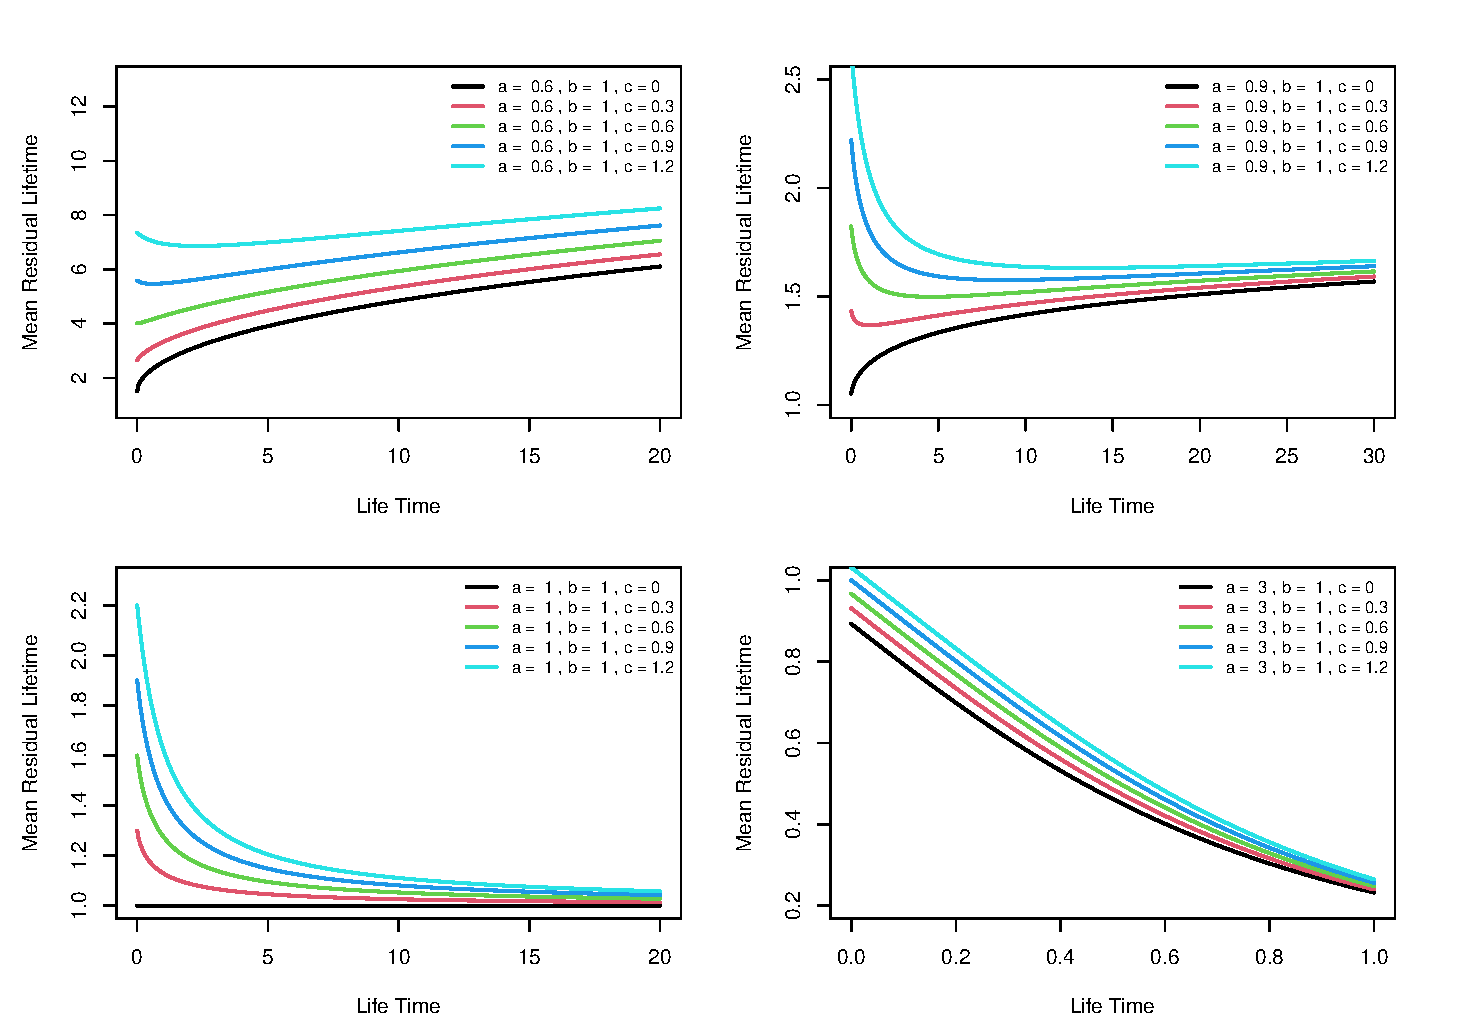
\includegraphics[width=10cm,height=9cm]{Figure41.eps}
	\caption{For fixed a and b, as c increases, the mean residual lifetime also increases.}
	\label{Figure41}
\end{figure}

\begin{figure}[h!]
	\centering	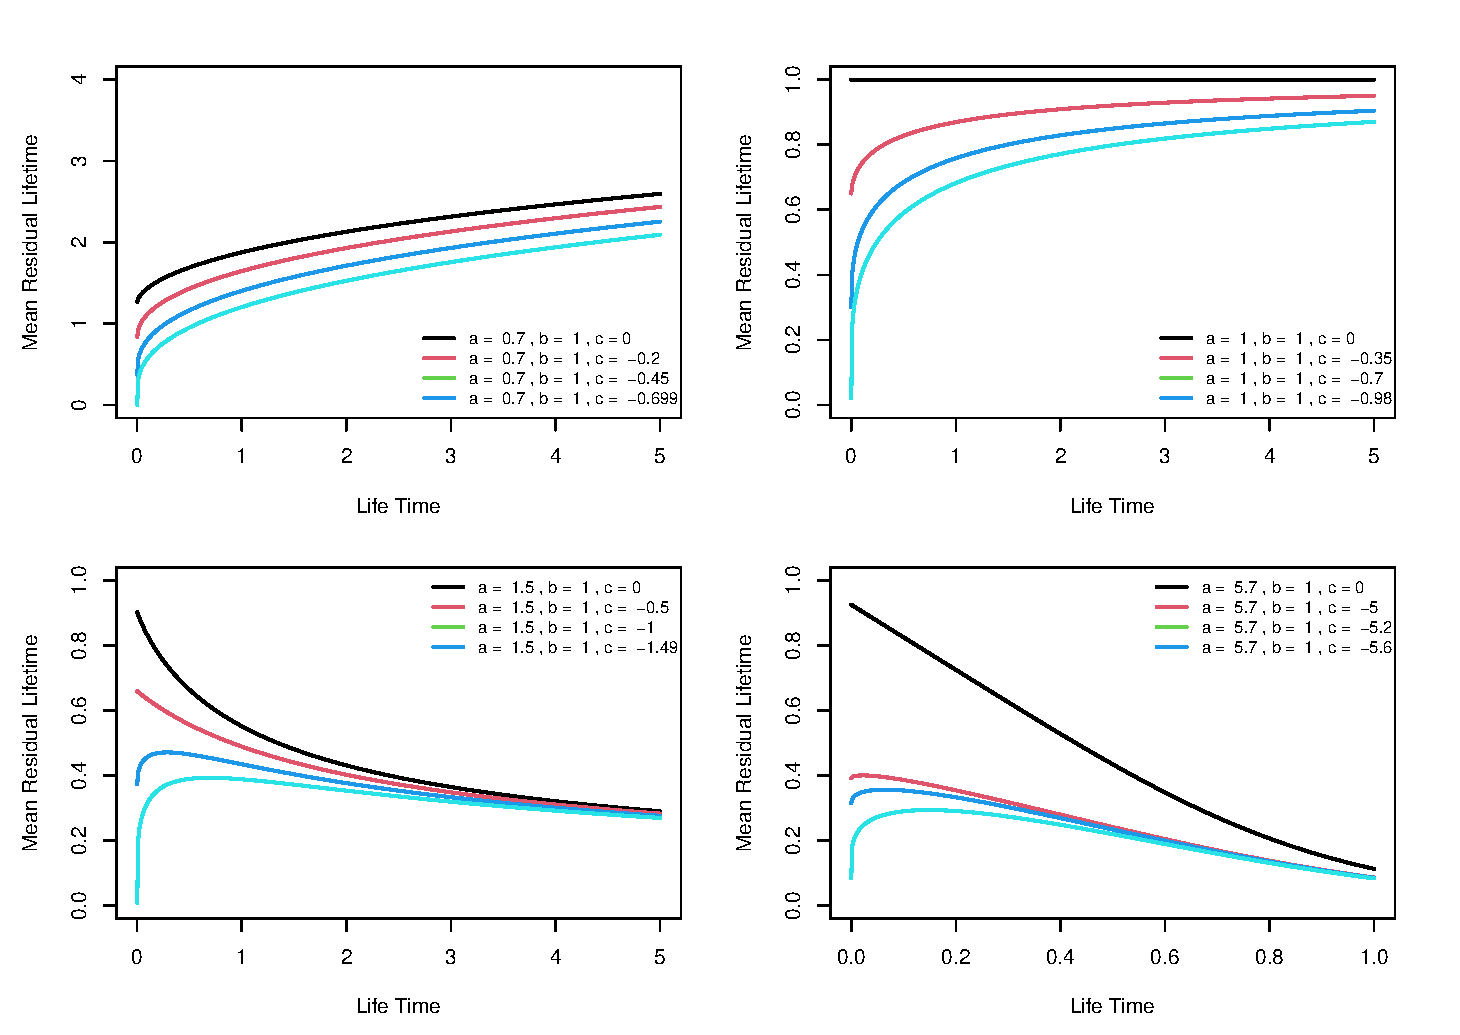
\includegraphics[width=10cm,height=9cm]{Figure51.eps}
	\caption{For fixed a and b, as c decreases, the mean residual lifetime also decreases.}
	\label{Figure51}
\end{figure}

It turns out that, from Figures \ref{Figure41} and \ref{Figure51}, the MRL is increasing in terms of the gamma shape parameter for Weibull shape and scale parameters.


\section{Kullback-Leibler Divergence }\label{sec05:information-analysis}

Kullback-Leibler \cite{Kullback-Leibler} divergence (i.e., relative entropy) defines a natural “statistical distance” to measure the discrepancy between two distributions. We are particularly interested in the discrepancy between the $GG (a, b, c)$ distribution and the standard Weibull distributions $GG(a, b, 0)$. In this section, we define a Kullback-Leibler divergence and obtain some theoretical results of the "distance" in relation to the gamma shape parameter $c$. 


For any given two continuous distributions $f_1$ and $f_2$, the Kullback-Leibler divergence is defined to be



\begin{equation}\label{KL-dist}
	KL[f_1||f_2] = \int_{D_1}f_1(x)\ln\left[ \frac{f_1(x)}{f_2(x)} \right] dx,
\end{equation}
\noindent where $D_1$ is the domain of $f_1(x)$.

We first derive the KL divergence based on the GG model with parametrization (\ref{new-GG-pdf}). We denote $GG_1(a_1, b_1, c_1)$ and $GG_2(a_2. b_2, c_2)$ to be two different GG distributions. The KL divergence between the two GG distributions is given below.

\begin{lemma}\label{lemma5.1}
	Assume that $GG_1(a_1, b_1, c_1)$ and $GG_2(a_2. b_2, c_2)$ are two generalized gamma distributions. The Kullback-Leibler divergence measure between any two GG distributions is given by        
	$$
	KL[f_{GG_1}||f_{GG_2}] = \ln \frac{\Gamma[p_2/a_2]a_1b_1^{-p_1}}{\Gamma[p_1/a_1]a_2b_2^{-p_2}} + \frac{p_1-p_2}{a_1}\left[ \Psi\left(\frac{p_1}{a_1} \right)+ \ln b_1\right]
	$$
	\begin{equation}
		-\frac{p_1}{a_1} + \left(\frac{b_1}{b_2} \right)^{a_2}\frac{\Gamma[(p_1+a_2)/a_1]}{\Gamma[p_1/a_1]}
	\end{equation}
	\noindent where $p_1 = a_1 + c_1$ and $p_2 = a_2 + c_2$.
\end{lemma}

\begin{proof}
	The proof is given in the appendix.	
\end{proof}

Let $g_0(x)$ and $g_1(x)$ be the density functions of the standard Weibull and the generalized gamma distributions, denoted by $GG(a,b,0)$ and  $GG(a, b, c)$, respectively. The Kullback-Leibler divergence measures $KL[g_0||g_1]$ and $KL[g_1||g_0]$ are given respectively by
\begin{equation}
	KL[g_0||g_1] = \ln \Gamma[(a+c)/a] + c\ln b - \frac{c}{a}[\Psi(1)+ \ln b],
\end{equation}
\noindent and
\begin{equation}
	KL[g_1||g_0] = \frac{c}{a}\left[\Psi[(a+c)/a] +\ln b\right] - \ln\Gamma[(a+c)/a] - c\ln b.
\end{equation}
Since $KL[g_0||g_1]$  and $KL[g_1||g_0]$  are not equal. It is better to define asymmetric distance using both KL divergence measures. We choose to define a measure to assess the discrepancy between the generalized gamma and the Weibull distribution by taking the sum of the two Kullback-Leibler divergence measures as follows
\begin{equation}
	D_{(g_0, g_1)}(c) = KL[g_0||g_1] + KL[g_1||g_0] = \frac{c}{a}\left[ \Psi\left(\frac{a+c}{a} \right) - \Psi(1)\right]
\end{equation}
The KL divergence measure as a function of gamma shape parameter $c$, $D_{(g_0, g_1)}(c)$,  provides a way to describe how the gamma shape parameter $c$ impacts the discrepancy between the Weibull and the generalized gamma distributions.
\begin{theorem}\label{thm5.2}
	Let $g_0(x)$ and $g_1(x)$ be the density functions of the standard Weibull distribution $GG(a, b, 0)$ and the generalized gamma distribution $GG(a, b, c)$, respectively. The distance $D_{(g_0, g1)}(c)$  measuring the discrepancy between  $g_0(x)$ and $g_1(x)$  has the following properties:\\
	(a).  $D_{(g_0, g1)}(c)$ is a non-negative function of $c$ for all $a$. \\
	(b).  $D_{(g_0, g1)}(c)$ is a decreasing function on $(-a, 0)$ and an increasing on $(0, \infty)$.\\
	(c).  $D_{(g_0, g1)}(c) = 0$ if and only if $g_0(x) = g_1(x)$.
\end{theorem}
\begin{proof}
	(a). Note that $\Psi()$ is an increasing function. If $c > 0$, $(a + c)/a > 0$ which implies that $\Psi[(a+c)/a] > \Psi(1)$. Therefore, $D_{(g_0, g_1)} > 0$. This result holds for the case of $c < 0$ using a similar argument.	\\
	(b). We use the properties of polygamma functions in Lemma \ref{lemma3.1} to prove this part. Taking the derivative of $D_{(g_0, g_1)}(c)$, we have
	$$
	\frac{d D_{(g_0, g_1)}(c)}{d c} = \frac{\Psi[(a+c)/a]-\Psi(1)}{a} + \frac{c\Psi_1[(a+c)/a]}{a^2}.
	$$
	Note that $\Psi[(a+c)/a] > 0$ for $c > - a$.\\
	
	\noindent \emph{Case 1}: If $c \in (-1, 0)$, then $\Psi[(a+c)/a] - \Psi(1) < 0$  since digamma is increasing (Lemma \ref{lemma3.1}). This means $d D_{(g_0, g_1)}(c)/d c < 0$. Hence, $D_{(g_0, g_1)}(c)$  is a decreasing function on $(-a, 0)$. \\
	
	\noindent \emph{Case 2}: If $c \in (0, \infty)$, then $\Psi[(a+c)/a] - \Psi(1) > 0$ . Therefore,  $d D_{(g_0, g_1)}(c)/d c > 0$. This means that $D_{(g_0, g_1)}(c)$ is increasing on $(0, \infty)$. \\
	
	From the above cases 1 and 2, we know that $c = 0$ is the unique root of equation $d D_{(g_0, g_1)}(c)/d c = 0$ .  Note that
	$$
	\frac{d^2D_{(g_0, g_1)}(c)}{d c^2}\left| _{c=0} \right.=\left\{\frac{2\Psi_1[(a+c)/a]}{a^2}+\frac{c\Psi_2[(a+c)/a]}{a^3} \right\} \left| _{c=0} \right. = \frac{2\Psi_1(1)}{a^2} > 0.
	$$
	Therefore, $D_{(g_0, g_1)}(c)$ is a convex function achieving the minimum at $c = 0$.\\
	
	\noindent (c). The sufficient condition is obvious. We only prove the \emph{necessary condition}. Assume that $D_{(g_0, g_1)}(c) = c\left\{ \Psi[(a+c)/a] -\Psi(1)\right\}$, then c = 0 or   $\Psi[(a+c)/a]-\Psi(1)= 0$. The second equation implies $c = 0$ since digamma function is strictly increasing. This proves that $g_0 \equiv g_1$, hence, the necessary condition holds.   
\end{proof}

\begin{figure}[h!]
	\centering	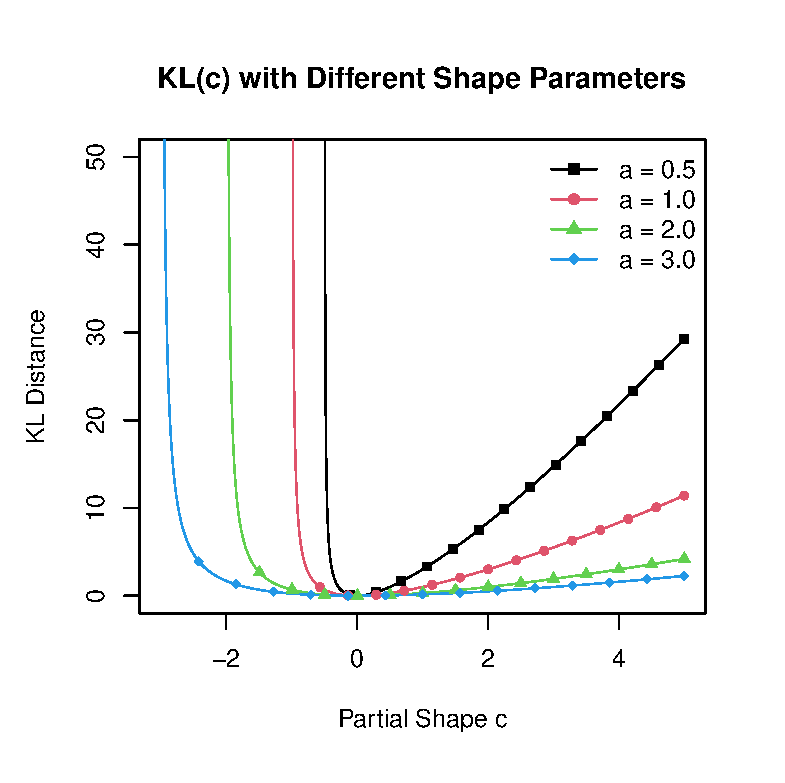
\includegraphics[width=8cm,height=7cm]{Figure06_KL_dist.eps}
	\caption{KL distance as a function of gamma shape parameter $c$ with different values of the shape parameter $a$. }
	\label{Figure06_KL_dist}
\end{figure}


Part (c) of the above theorem will be used to develop a parametric hypothesis test for $H_0: c = 0$ in Section \ref{sec07:asymp-tests}.


\section{Maximum Likelihood Estimation and Inference}\label{sec06:MLE}

This section focuses on the maximum likelihood estimation of the model parameters and relevant inferences.

\subsection{Likelihood function under reparametrization}\label{sec6.1: reparametrization}

To avoid computational challenges, we reparametrize the model parameter by letting $p = a + c$.  The three parameters after reparametrization are $a$, $b$, and $p$. 
\begin{equation}\label{reparametrization}
	g(x)=\frac{(a/b)(x/b)^{p-1}\exp[-(x/b)^a]}{\Gamma(p/a)}.
\end{equation}

The inference on the partial gamma shape parameter c will be based on $c = p-a$.  Next, we establish the maximum likelihood estimation of the model parameters $a$, $b$, and $p$.  For notational convenience, we denote $GG^S(a,b,p) = GG(a, b, a+c)$ to reflect the reparametrization (where $p = a + c$). With this new notation, the two-parameter Weibull is represented by $GG(a, b, 0) = GG^S(a, b, a)$ and the two-parameter gamma distribution is  $GG(1, b, c) = GG^S(1, b, 1+c)$.\\

Let $\{x_1, x_2, \cdots, x_n \}$ be a random sample taken from the population that follows the proposed GG distribution. The likelihood function has the following form
\begin{equation}\label{likelihood-fun}
	L(a,b,p) = \prod_{i=1}^n g(x_i)=\left[\Gamma(p/a) \right]^{-n} (a/b)^n\prod_{i=1}^n\left\{
	(x_i/b)^{p-1}\exp\left[- (x_i/b)^a\right]\right\}.
\end{equation}
The log-likelihood function is given by
\begin{equation}\label{log-likelihood-fun}
	l(a,b,p) = n\ln a -n\ln b -n\ln \Gamma(p/a) + (p-1)\sum_{i=1}^n \ln (x_i/b) -\sum_{i=1}^n (x_i/b)^a.
\end{equation}
The log-likelihood involves the log gamma function. We have studied some properties of the log gamma functions and their derivatives in Section \ref{sec03:pdf-shape}.


\subsection{MLE of model parameters and asymptotic results}\label{sec6.2:mle-asymp}

With the above notations, we derive the score equations as follows
\begin{subequations}
	\begin{equation}
		\frac{\partial l(a,b,p)}{\partial a} = \frac{n}{a} + \frac{np}{a^2}\Psi\left(\frac{p}{a}\right)-\sum_{i=1}^n\left( \frac{x_i}{b}\right)^a\ln \left( \frac{x_i}{b}\right) = 0,
	\end{equation}
	\begin{equation}
		\frac{\partial l(a, b, p)}{\partial b} = -\frac{np}{b} + \frac{a}{b}\sum_{i=1}^n \left( \frac{x_i}{b}\right)^a = 0,
	\end{equation}
	\begin{equation}
		\frac{\partial l(a, b, p)}{\partial p} = -\frac{n}{a}\Psi\left(\frac{p}{a}\right) + \sum_{i=1}^n \ln\left( \frac{x_i}{b}\right) = 0.
	\end{equation}
\end{subequations}

The MLE of $\theta = c(a, b, p)^T$, denoted by $\hat{\theta}=c(\hat{a}, \hat{b}, \hat{p})^T$, is the solution to the above score equations.	

To derive the asymptotic results of the MLE, we need the following Fisher information matrix (of the sample) that is defined to be the expectation of the Hessian matrix $H(\theta)$ with the following form
\begin{equation}
	I_n(\theta) = -E[H(\theta)] = -E\begin{bmatrix}
		\frac{\partial^2 l(\theta)}{\partial a^2} & \frac{\partial^2 l(\theta)}{\partial a \partial b} & \frac{\partial^2 l(\theta)}{\partial a \partial p} \\
		\frac{\partial^2 l(\theta)}{\partial b\partial a} & \frac{\partial^2 l(\theta)}{\partial b^2} & \frac{\partial^2 l(\theta)}{\partial b \partial p} \\
		\frac{\partial^2 l(\theta)}{\partial p\partial a} & \frac{\partial^2 l(\theta)}{\partial p\partial b} & \frac{\partial^2 l(\theta)}{ \partial p^2}
	\end{bmatrix}
	=\begin{bmatrix}
		i_{a^2} & i_{ab} & i_{ap} \\
		i_{ba} & i_{b^2} & i_{bp} \\
		i_{pa} & i_{pb} & i_{p^2} 
	\end{bmatrix}
\end{equation}
\noindent where $\theta = (a, b, p)$. After some algebra, we have the following explicit expression of the cell elements of the Fisher Information matrix (of the sample data).
$$
i_{aa}=\frac{n}{a^2} \left[\left(\frac{p}{a}\right)^2\Psi_1\left(\frac{p}{a} \right)+1\right]
+\frac{np}{a^3}\left[\Psi^2\left(\frac{a+p}{a} \right)+2\Psi\left(\frac{p}{a}\right)+\Psi_1\left(\frac{a+p}{a} \right) \right]
$$
$$
i_{ab} =-\frac{np}{ab}\left[ \Psi\left(\frac{a+p}{a}\right) +1\right] ,\hspace{5mm}
i_{ap} = -\frac{n}{a^2}\left[ \Psi\left(\frac{p}{a} \right)+\frac{p}{a}\Psi_1\left( \frac{p}{a}\right)\right]
$$
$$
i_{bb}= \frac{npa}{b^2},  \hspace{5mm} i_{bp} =  \frac{n}{b},  \hspace{5mm} i_{pp} =  \frac{n}{a^2}\Psi_1\left( \frac{p}{a}\right)
$$

The asymptotic results of MLE can be established under some regularity conditions (such as parameter space is invariant on sample size, the likelihood function is continuous, and the first three moments are bounded) based on the following theorem. 

\begin{theorem}
	Let $\hat{\theta} = (\hat{a}, \hat{b}, \hat{p})$ be the MLE of the true parameter $\theta=(a, b, p)$ estimated based on the i.i.d. sample $\{ x_1, x_2, \cdots, x_n\}$ from the GG model and $T(\theta)$ be the expected Fisher Information matrix. The asymptotic sampling distribution of $\hat{\theta}$ is given by	
	\begin{equation}\label{asymp-dist-MLE}
		(\hat{\theta}-\theta) \to N\left(0, I_n^{-1}(\theta)\right)
	\end{equation}
\end{theorem}


For convenience, we denote
\begin{equation}\label{covariance-matrix}
	\mbox{var}(\hat{\theta}) = I^{-1}(\theta)=
	\begin{bmatrix}
		\sigma_{aa}(\theta) & \sigma_{ab}(\theta) & \sigma_{ap}(\theta) \\
		\sigma_{ba}(\theta) & \sigma_{bb}(\theta) & \sigma_{bp}(\theta) \\
		\sigma_{pa}(\theta) & \sigma_{pb}(\theta) & \sigma_{pp}(\theta)
	\end{bmatrix}
\end{equation}

The MLE of the variance is obtained using the plug-in principle of MLE, that is, $\widehat{\mbox{var}}(\hat{\theta}) = I^{-1}(\hat{\theta})$. In general, if the closed form of the Information matrix does not exist or the approximation of the matrix is hard to obtain or too complex, we can use the observed Fisher Information matrix (i.e., negative Hessian matrix) in many practical applications. In this study, we have a closed form of the Fisher information matrix that is easy to evaluate. Both the observed information matrix and the observed Fisher information matrix can be used in practical applications.


\section{Goodness-of-fit and Model Selection}\label{sec07:asymp-tests}


Two major types of tests of particular interest will be discussed in this section: a goodness-of-fit test of GG and tests for testing the discrepancy between the GG and the standard Weibull models.


\subsection{Kolmogorov–Smirnov Test}\label{sec7.1:KS-test}

To test the goodness of fit of the model, we propose the Kolmogorov–Smirnov (KS) test which is defined based on the distance between the CDFs of the GG and its empirical distributions based on the random sample. The test statistic is defined by



\begin{equation}
	D_n=\sqrt{n} \sup_{x\in R^+} |GG_n(x) - GG_0(x)|, 
\end{equation}
\noindent where the empirical CDF is defined as $GG_n(x) = \sum_{i=1}^n I(x_i<x)/n$ using the random sample and $G_0(x)$ is the CDF of GG specified in (\ref{new-GG-CDF}). Consider testing hypothesis
$$
\mbox{H}_0:\hspace{3mm} GG = GG_0 \hspace{5mm}\mbox{v.s.}\hspace{5mm}\mbox{H}_1:\hspace{3mm} GG \ne GG_0
$$
Under the null hypothesis, the above test statistic follows (approximately) Kolmogorov-Smirnov distribution with CDF
$$
F_{KS}(x) = 1 -\sum_{k=1}^n(-1)^{k-1}\exp(-2k^2x).
$$
Let $q$ be a real number determined by the significance level $\alpha$, that is, $q$ satisfies
$$
\alpha = P[D_n \ge q | H_0].
$$
The decision of the KS test is based on the following rule:  
\begin{equation}
	\mbox{Ho is concluded if } D_n \le q; \hspace{3mm}\mbox{Ho is rejected if } D_n > q.
\end{equation}


\subsection{A Monte Carlo Goodness of Fit}\label{KL-Test}

In this subsection, we propose a Monte Carlo KLD test to justify the discrepancy between the generalized gamma and the standard Weibull models. Let $g_1(x)$ be the density function of the three-parameter generalized gamma distribution $GG(a, b, c)$ and $g_0(x)$ be the two-parameter Weill distribution $GG(a, b, 0)$. In Section \ref{sec05:information-analysis}, we defined the KLD between  $GG(a, b, c)$ and $GG_0(a, b, 0)$ using Stacy’s \cite{Stacy-1962} original parametrization as follows
\begin{equation}\label{KL-statistic}
	D_{(g_0, g_1)}(p,a) = \frac{p-a}{a}\left[\Psi(p/a)-\Psi(1) \right]
\end{equation}
\noindent where $p = a + c$. 

Intuitively, if the gamma shape parameter $c$ in a generalized gamma distribution is zero, then $D_{(g_0, g_1)}(p,a) = 0$. Empirically, if we fit the three-parameter generalized gamma model $GG(a, b, c)$ to a random sample $\{x_1, x_2, \cdots, x_n\}$ to obtain MLE $(\hat{a}, \hat{b}, \hat{c})$ and plug $\hat{a}$ and $\hat{p} = \hat{a} + \hat{c}$ into $D_{(g_0, g_1)}(p,a) = 0$, denoted as $\widehat{KLD} = D_{(g_0, g_1)}(\hat{p},\hat{a})$. If $\widehat{KLD}$ is significantly bigger than zero, we have evidence to claim the underlying population is NOT a Weibull distribution. Otherwise, we support the underlying population to be the regular two-parameter Weibull. Therefore, $\widehat{KLD} = D_{(g_0, g_1)}(\hat{p},\hat{a})$ can be used to establish a formal testing hypothesis about  

\begin{equation}\label{MC-test}
	H_0: GG = GG(a,b,0)  \hspace{5mm} \mbox{versus} \hspace{5mm}  H_a: GG = GG(a, b, c)
\end{equation}

In order to find the p-value for making a statistical decision, we need to know the distribution of  $\widehat{KLD}$. The analytical (asymptotic) sampling distribution is not available due to the definition of the KLD. However, we can easily simulate the sampling distribution of the test statistic (i.e., the estimated KLD) via the Monte Carlo method. The following algorithm gives the steps for this test.\\

\noindent {\bf Algorithm 7.1.} \emph{The steps for performing the Monte Carlo test (\ref{MC-test}) are given in the following.}\\
\noindent A. \emph{{\bf Test Statistic}: Let $\{ x_1, x_2, \cdots, x_n\}$ be the random sample from $GG^S(a, b, p)$ (Stacy's parametrization) and $(\hat{a}, \hat{b}, \hat{p})$ be the MLE of $(a, b, p)$. Plug $(\hat{a}, \hat{b}, \hat{p})$ into (\ref{KL-statistic}) to find the test statistic}  

\begin{equation}\label{TS}
	TS = \frac{\hat{p}-\hat{a}}{\hat{a}}\left[\Psi(\hat{p}/\hat{a})-\Psi(1) \right]
\end{equation}
\noindent B. \emph{{\bf Sampling Distribution of TS under H\textsubscript{0}}:\\ 
	B.1. Generate B Monte Carlo random samples with the same size as the data set from Weibull distribution $GG^S(\hat{a}, \hat{b}, \hat{a})$. \\
	B.2. Fit the three-parameter generalized gamma $GG^S(a, b, p)$ to each of the B samples and obtain MLEs $(\tilde{a}_m, \tilde{b}_m, \tilde{p}_m)$ for $m = 1, 2, \cdots, B$. \\
	B.3.Using each set of MLEs obtained from each Monte Carlo sample to evaluate the Monte Carlo test statistic, for $m =1, 2, \cdots, B$; }
\begin{equation}\label{TS-MC}
	\widetilde{TS}_m = \frac{\tilde{p}_m-\tilde{a}_m}{\tilde{a}_m}\left[\Psi(\tilde{p}_m/\tilde{a}_m)-\Psi(1) \right]
\end{equation}
B.4. The sampling distribution of the test statistic can be approximated by the following Monte Carlo sampling distribution based on $\{\widetilde{TS}_1, \widetilde{TS}_2, \cdots, \widetilde{TS}_B \}$.\\

\noindent C. \emph{{\bf P-value of Monte Carlo Test}: The p-value can be calculated by  
	\begin{equation}\label{MC-p-value}
		\mbox{p-value} \approx \#(\widetilde{TS}_m  > TS)/B.
	\end{equation}
}
\begin{remark}
	
	The KLD has a nice analytic expression. However, we cannot use the plug-in principle of the MLE to approximate the sampling distribution of the test statistics, $\widehat{KLD}$, under $H_0$ since the two hypothetical distributions were assumed to have the same (Weibull) shape $a$ and the same scale $b$ and $p = a$. In other words, the null hypothesis does not claim any specific values for the parameters. Therefore, the delta method cannot be used to approximate the distribution of $\widehat{KLD}$ based on the asymptotic distribution of $(\hat{a}, \hat{b}, \hat{p})$.
	
\end{remark}



\section{Simulation Studies and Power Analysis}\label{sec08:Simulation}

We introduced a simulation-based Monte Carlo test for the gamma shape parameter using KLD in Section \ref{sec07:asymp-tests}. In this section, we perform a small simulation study to evaluate the performance of the proposed test.  We choose the values of the Weibull shape and scale parameters to be $a = 4$, $b = 2$, respectively. The gamma shape parameter  $c = -3.5, -3.2, -3, -2.6, -2.5, -2.0, -1.5, -1, -0.5, 0, 1, 1.2, 1.5, 1.8, 2, 2.5, 2.8, 3, 3.3, 3.5$. We also choose 4 different sample sizes $n = 30, 50, 100, 200$ to see how the sample size impacts the power. 

\subsection{GG random number generation}\label{random-generation}

For each combination of $(a, b, c)$, we simulated 1000 Monte Carlo samples from $GG(a, b, c)$ using the relationship between the generalized gamma and the specific gamma distributions specified in (\ref{quantile-fun}).  To be more specific, we summarize the following steps for generating the random number from the generalized gamma distribution with given values for the model parameters.\\


\noindent \emph{{\bf Algorithm 8.1}. Let $q(u) = \mbox{qgamma}(u, \mbox{shape}, \mbox{scale})$ be the quantile function of the regular gamma distribution and be available in an existing program such as R, Python, and SAS. To generate a random number from $GG(a, b, c)$,}\\

\noindent \emph{{\bf A.} Generate a random number from uniform distribution} $u = \mbox{unif}(0,1)$.\\
\noindent \emph{{\bf B.} The following}
$$X = b\left(\mbox{qgamma}\left[ u, \mbox{shape}=\frac{a + c}{a}\right]\right)^{1/a}$$
\noindent \emph{is the desired random number from $GG(a, b, c)$.}\\

To simulate the Monte Carlo distribution of the KLD under the null hypothesis of the Weibull distribution (we also call it \emph{null distribution} of $\widehat{KLD}$), we simply simulate $B$ random samples with the sample size used in the simulation from $GG(a, b, 0)$ explicitly using $b\left(\mbox{qgamma}\left[ u, \mbox{shape}=1\right]\right)^{1/a}$ (with $u$ from Unif$[0,1]$). 


\subsection{Power analysis}\label{power-analysis}

To calculate the power of the Monte Carlo test using various alternatives that are only dependent on the different values of the gamma shape parameter and four different sample sizes mentioned earlier.

For the null distribution, we simulate 10000 Weibull standalone samples from $GG(a, b, 0)$ to approximate the sampling distribution of $\widehat{KLD}$ under the null hypothesis $H_0: c = 0$. 

For each combination of gamma shape parameter $c$ and sample size $n$, we simulate 10000 random samples from $GG(a, b, c)$ and calculate the corresponding KLD. The significant level is 0.05.

The simulated power curves are summarized in the following figure.

\begin{figure}[h!]
	\centering	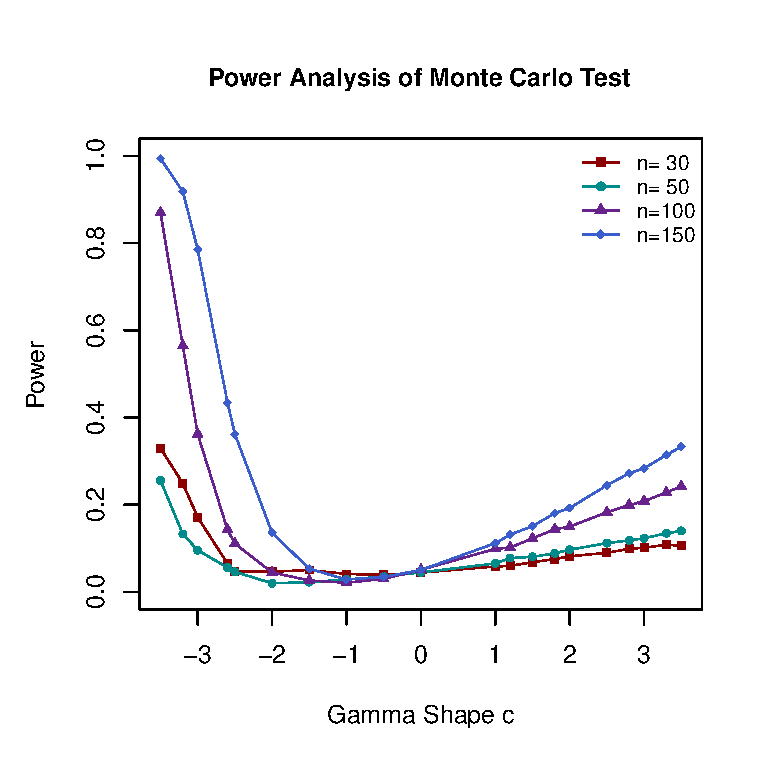
\includegraphics[width=8cm,height=7cm]{Figure07_power_analysis.eps}
	\caption{Power curves of the Monte Carlo test with different $c$ and sample size $n$. }
	\label{Figure07_power_analysis}
\end{figure}

\noindent As anticipated, we can see the following patterns from the above power curves.\\
(1). The power of the Monte Carlo test at $c = 0$ is close to the nominal level of 0.05.\\
(2). As $c$ deviates from 0, the power of the underlying test gets bigger except for some negative $c$ values that are close to 0.\\
(3). As sample size increases, the corresponding power increases for any fixed value of $c$ except for some negative values of $c$ that are close to 0.

\section{Real-World Applications}\label{sec09:Numerical-examples}

The primary focus of this section is two-fold. The first objective is to perform a Kolmogorov–Smirnov goodness-of-fit test to determine whether the sample data in each example came from the generalized gamma family. The second objective is to perform significant tests on the two shape parameters $H_0: a = 1$ (i.e., the two-parameter gamma distribution) and $H_0: c = 0$ (i.e., the two-parameter Weibull distribution) to possibly select an appropriate subfamily of the GG to avoid potential over-fitting / under-fitting issues. In addition to using the standard Wald $\chi^2$ significance test for the two shape parameters, we use the proposed Monte Carlo simulation-based test for the new gamma shape parameter $c$. Testing for $H_0: b = 1$ is provided for practitioners to potentially choose a simpler model in the GG family. 


\subsection{Environmental Process Modeling}

{\bf Example 1}. We use the average flows of water (in m$^3$/s) of the Piracicaba River, Brazil, between August 1972 and 2014. The data sets were obtained from the Department of Water Resources and Power agency manager of water resources of the State of S$\tilde{a}$o Paulo by Ramos et al  \cite{Ramos-et-al-2021}.  Accurately estimating the distribution of the water flow is essential for environmental planning and policymaking to meet the needs of people, agriculture, industry, energy, and ecosystems within the limits of available supply and under a changing climate. Environmental flow is a practical tool for managing allocation in the water-energy-food nexus. We only use the August data to fit the GG to the data and report the results of tests in the following table.

\begin{center}
\begin{table}[h!]
	\caption{Results of various tests for the average water flow data of Piracicaba River, Brazil. }
	{\begin{tabular}{lcccc} \hline
			Test                & MLE      &   SE      &  TS        & P-value         \\ \hline
			$H_0$: a = 1 (Wald) & 0.49818  & 0.02166   & 536.9969   & $< 0.0001$      \\
			$H_0$: b = 1 (Wald) & 0.00382  & 0.00049   &  4225061   & $< 0.0001$      \\
			$H_0$: c = 0 (Wald) & 24.399   & 4.6613332 & 27.39862   & $< 0.0001$      \\ 
			$H_0$: c = 0 (MC)   &   --     &   --      &    --      & $\approx 0.004$ \\ 
			$H_0$:  GOF (K-S)   &   --     &   --      & 0.15563    & 0.24692         \\
			\hline
	\end{tabular}}
	%\tabnote{\textsuperscript{a} Kolmogorov-Smirnov Test - $H_0$: the underlying distribution is a generalized gamma distribution.\\ \textsuperscript{b} Bootstrap KLD test for $H_0$: c = 0.}
	\label{Environmental-data}	
\end{table}
\end{center}

The result of the KS test in Table \ref{Environmental-data} implies that the sample comes from a generalized gamma population (p-value = 0.247). Both Wald and Monte Carlo significance tests of the shape parameters indicate that the gamma and Weibull distributions are inappropriate in modeling this water flow data. The generalized gamma distribution is appropriate for modeling the average of the water flow.

\subsection{Modeling Financial Volatility }

{\bf Example 2}.  As a measure of risk, volatility plays an important role in both asset pricing and risk management and has been a central theme in the literature of both financial economics and econometrics. The popular exponential and Weibull distributions are commonly used for estimating volatility. However, misspecification of the distribution for the volatility causes serious modeling issues such as inlier and outlier problems in volatility forecasting (see Xie and Wu's \cite{Xie-Wu-2017} recent work for more detail). 


The data set for this example is taken from the recent work of Afuecheta et al \cite{Afuecheta-2020} in which authors proposed several candidate innovations for the GARCH model to predict the volatility of financial series. The returns data of Litecoin (LTC) for the period starting from the 24th of October 2013 to the 16th of June 2018 will be used in this example. The volatility is measured by the standard deviation of daily log-returns of Litecoin (LTC) taken over non-overlapping windows of a length of 30 days (a 50-day window was used in the original paper). To avoid rounding-off errors due to the small magnitude of volatility, we re-scale the volatility by multiplying 100 before fitting the gamma distribution to re-scaled data. The following table summarizes the test results. 

\begin{center}
\begin{table}[h!]
	\caption{Results of various tests for Litecoin returns data. }
	{\begin{tabular}{lcccc} \hline
			Test                & MLE     &   SE    &  TS      & P-value         \\ \hline
			$H_0$: a = 1 (Wald)     & 0.36435 & 0.01788 & 1263.4   & $< 0.0001$      \\
			$H_0$: b = 1 (Wald)     & 0.00388 & 0.00109 & 835403.7 & $< 0.0001$      \\
			$H_0$: c = 0 (Wald)     & 4.71687 & 0.73862 & 40.8     & $< 0.0001$      \\
			$H_0$: c = 0  (MC)      &   --    &   --    &   --     & $< 0.023$      \\  
			$H_0$: GOF   (K-S )     &   --    &   --    & 0.065995 & 0.9677          \\ 
			\hline
	\end{tabular}}
	\label{Financial-risk-data}
\end{table}
\end{center}


The results in Table \ref{Financial-risk-data} indicate that the generalized gamma distribution fits the 30-day volatility of LTC daily log returns appropriately. The large sample Wald and Monte Carlo simulation tests indicate that both gamma and the Weibull distribution are inappropriate for modeling the returns of LTC because of the underfitting issue. Therefore, to avoid misspecification, the generalized gamma distribution should be used to estimate the volatility in this study. 


\section{Discussions and Conclusions}\label{sec10:conclusion}

We provide a new formulation of the well-known generalized gamma distribution by adding an additive gamma shape parameter $c$ to the regular two-parameter Weibull distribution. Some novel characterizations of the shape of the hazard rate and density curves associated with the gamma parameter $c$ are provided. These shape characterizations are useful in many applications such as in modeling statistical processes for capability and quality control, the behavior of hazard rates in reliability, and survival analysis.   

We also developed a novel Monte Carlo simulation test using Kullback-Leibler divergence-based (KLD) for model selection between the standard Weibull distribution and generalized gamma distribution. Several other tests for goodness-of-fit and significance of the two shape parameters to avoid potential model misspecification and over/under-fitting issues were also presented. 

The two real-world numerical examples demonstrate that, in some real-world application problems, the generalized gamma distribution must be used to avoid potential under-fitting, while in some other applications, distributions in a sub-family of the generalized gamma such as Weibull, gamma, or exponential must be used to avoid over-fitting. 


\section*{Acknowledgments}

\begin{acknowledgement}
The author sincerely thanks an anonymous reviewer for careful reading of the manuscript and for insightful comments and suggestions that improved the presentation of this work.   
\end{acknowledgement}


\section*{Data Availability Statement}

The code used in this paper is available online in a GitHub repository: https://github.com/pengdsci/GG \cite{Peng-2023}.


%\section*{Funding}

%\section*{Notes on contributor(s)}

%\section*{Nomenclature/Notation}

%\section*{Notes}


%\section{References}
\begin{thebibliography}{}
	
	\bibitem{Afuecheta-2020}
	E. Afuecheta, A. Semeyutin, S. Chan, S. Nadarajah, D. A. P. Ruiz, \emph{Compound distributions for financial returns}, PLoS ONE, 15(2021), doi: 10.1371/journal.pone.0239652.
	
	\bibitem{Allenby-Leone-Jen-1999}	
	G. M. Allenby, R. P. Leone , and L. Jen,  \emph{A dynamic model of purchase timing with application to direct marketing}, Journal of the American Statistical Association, 94 (1999), pp. 365--374.
	
	\bibitem{Almalki-Nadarajah-2014}
	S. Almalki  and S. Nadarajah,  \emph{Modifications of the Weibull distribution: A review}, Reliability Engineering \& System Safety, 124 (2014), pp. 32--55.
	
	\bibitem{Alzer-1997}
	H. Alzer, \emph{On Some Inequalities for the Gamma and Psi Functions}, Mathematics of Computation,  66 (1997), pp. 373--389.
	
	\bibitem{Balakrishnan-Pal-2015}
	N. Balakrishnan and S. Pal,  \emph{An EM algorithm for the estimation of parameters of a flexible cure rate model with generalized gamma lifetime and model discrimination using likelihood- and information-based methods}, Computational Statistics, 30 (2015),  pp. 151--189.
	
	\bibitem{Bebbington-Lai-Zitikis-2007}
	M., Bebbington, C. D. Lai and  R. Zitikis,  \emph{A flexible Weibull extension. Reliability Engineering and System Safety}, 92 (2007),  pp. 719--726.
	
	\bibitem{Bennette-1983}
	S. Bennette,  \emph{Log-logistic regression models for survival data}, Appl. Stat. 32 (1983), pp. 165--171.
	
	\bibitem{Carrasco-Ortega-Cordeiro-2008}
	J. M. F. Carrasco,   E. M. M.  Ortega, and G. M. Cordeiro,  \emph{A generalized modified Weibull distribution for lifetime modeling}. Computational Statistics and Data Analysis, 53 (2008),  pp. 450--462.
	
	%\bibitem{Cordeiro-Gomes-Da-Silva-Ortega-2013}
	%G. Cordeiro,  A. E. Gomes,  C. Q. Da-Silva,  and  E. M. Ortega, \emph{The beta exponentiated Weibull distribution}, Journal of Statistical %Computation and Simulation, 83(2003),  pp. 114--138.
	
	\bibitem{Dadpay-Soofi-Soyer-2007}
	A. Dadpay,  E. S. Soofi, and R. Soyer,  \emph{Information Measures for Generalized Gamma Family},  Journal of Econometrics, 138 (2007),  pp. 568--585.
	
	\bibitem{Diebold-Rudebusch-1990}
	F. X. Diebold and G. D. Rudebusch,  \emph{A Nonparametric investigation of duration dependence in the American business cycle},  Journal of Political Economy, 98 (1990),  pp. 596--616.
	
	\bibitem{Dodson-2006}
	B. Dodson,  \emph{The Weibull Analysis Handbook}, 2nd Edition, ASQ Quality Press. 2006.
	
	\bibitem{Efron-1988}
	B. Efron,  \emph{Logistic regression, survival analysis, and the Kaplan–Meier curve}, Journal of American Statistical Association, 83 (1988),  pp. 414--425.
	
	\bibitem{Gauss-Cordeiro-Lima-Gomes-Silva-Ortega-2016}
	M. Gauss, G. M. Cordeiro,  M. C. Lima,   A. E. Gomes, C. Q. Silva, and E. M. Ortega,  \emph{The gamma extended Weibull distribution}, Journal of Statistical Distributions and Applications, 2016 3:7
	
	
	\bibitem{Glaser-1980}
	R. E. Glaser  \emph{Bathtub and Related Failure Rate Characterizations}, Journal of the American Statistical Association, 75 (1980),  pp.667--672
	
	\bibitem{Gomes-Combes-Dussauchoy-2008}
	O. Gomes, C. Combes, and A. Dussauchoy,  \emph{Parameter estimation of the generalized gamma distribution}, Mathematics and Computers in Simulation 79 (2008),  pp.955--963
	
	\bibitem{Gradshteyn-Ryzhik-2007}
	I. S. Gradshteyn and I. M. Ryzhik,  \emph{Table of Integrals, Series, and Products}. Edited by A. Jeffrey and D. Zwillinger. Academic Press, New York, 7th edition, 2007.
	
	\bibitem{Guo-Feng-2013}
	B.-N. Guo and  Q. Feng, \emph{ Refinements of lower bounds for polygamma functions}, Proceedings of the American Mathematical Society, 141(2013),  pp. 1007--1015.
	
	\bibitem{Gupta-Viles-2013}
	R. C. Gupta and  W. Viles, \emph{ Roller-coaster failure rates and mean residual life functions with application to the extended generalized inverse gaussian models}, Probability in the Engineering and Informational Sciences, 25(2011),  pp. 103--118.
	
	\bibitem{Harter-1967}
	H.L. Harter,   \emph{Maximum-likelihood estimation of the parameters of a four-parameter generalized gamma population from complete and censored samples},  Technometrics, 9 (1967),  pp. 159--165.
	
	\bibitem{Kaniovski-Peneder-2008}
	S. Kaniovski and  M. Peneder,   \emph{Determinants of firm survival: a duration analysis using the generalized gamma distribution},  Empirica,  35 (2008),   pp. 41--58.
	
	\bibitem{Kullback-Leibler}
	S. Kullback and R. Leibler,  \emph{On information and sufficiency},  Ann. Math. Statist. 22 (1951),  pp. 79--86.
	
	\bibitem{Langlands-Pocock-Kerr-Gore-1979}
	A. O. Langlands,  S. J. Pocock,  G. R. Kerr,  and  S. M. Gore,  \emph{Long-term survival of patients with breast cancer: a study of the curability of the disease}. British Medical Journal, 2(1979),  pp. 1247--1251.
	
	\bibitem{Lai-2013}
	C.-D. Lai,  \emph{Generalized Weibull Distributions}, Springer Science \& Business Media. 2013.
	
	\bibitem{Lai-Xie-Murthy-2003}
	C. D. Lai,  M.  Xie and D. N. P. Murthy,  \emph{A modified Weibull distribution}. Transactions on Reliability, 52 (2003),  pp. 33--37.
	
	\bibitem{Lawless-1980}
	J. F. Lawless,   \emph{Inference in the Generalized Gamma and Log-Gamma Distributions}, Technometrics, 22(1980),  pp. 409--419. 
	
	\bibitem{McCool-2012}
	J. I. McCool,  \emph{Using the Weibull Distribution: Reliability, Modeling and Inference}. John Wiley \& Sons Inc. 2012.
	
	\bibitem{Medina-Moll-2009}
	L. A. Medina and V. H. Moll,  \emph{The integrals in Gradshteyn and Ryzhik-Part 10: The digamma function}, Scientia - Series A: Mathematical Sciences,  17 (2009),  pp. 45--66.
	
	\bibitem{Mudholkar-Srivastava-1993}
	G. S. Mudholkar and D. K. Srivastava,  \emph{Exponentiated Weibull family for analyzing bathtub failure-rate data}. IEEE Transaction on Reliability. 42 (1993), 299--302.
	
	\bibitem{Mudholkar-Srivastava-Freimer-1995}
	G. S. Mudholkar,   D. K. Srivastava and  M. Freimer,  \emph{The exponentiated Weibull family: a reanalysis of the bus-motor-failure data}. Technometrics. 37 (1995),  pp. 436--445.
	
	\bibitem{Mudholkar-Srivastava-Kollia-1996}
	G. S. Mudholkar,   D. K. Srivastava and G. D. Kollia,   \emph{A generalization of the Weibull distribution with application to the analysis of survival data}. Journal of American Statistical Association, 91 (1996),  pp. 1575--1583.
	
	\bibitem{Muqattash-Yahdi-2006}
	I. Muqattash and  M. Yahdi, \emph{Infinite family of approximations of the Digamma function}, Mathematical and Computer Modelling,  43 (2006), pp. 132--1336.
	
	\bibitem{Murthy-Xie-Jiang-2004}
	D. N. P. Murthy, M.  Xie  and R.  Jiang,  \emph{Weibull Models}, John Wiley \& Sons Inc. 2004.
	
	\bibitem{Nadarajah-Kotz-2005}
	S. Nadarajah and  S. Kotz, \emph{On some recent modifications of Weibull distribution}. IEEE Transaction on Reliability, 54 (2005),  pp. 561--562.
	
	\bibitem{Noufaily-Jones-2013a}
	A. Noufaily and M. C. Jones,  \emph{On maximization of the likelihood for the generalized gamma distribution}, Computational Statistics, 28 (2013a),  pp. 505--517.
	
	\bibitem{Noufaily-Jones-2013b}
	A. Noufaily and M. C. Jones,  \emph{Parametric quantile regression based on the generalized gamma distribution}, Journal of the Royal Statistical Society: Series C (Applied Statistics), 62 (2013b), 723--740.
	
	\bibitem{Ortega-Cordeiro-Kattan-2013}
	E. M. Ortega,  G. M. Cordeiro and M. W. Kattan,  \emph{The log-beta Weibull regression model with application to predicting recurrence of prostate cancer}, Statistical Papers, 54 (2013),  pp. 113--132.
	
	
	\bibitem{Peng-2023}
	Peng, C. R code for "A new formulation of generalized gamma: some results and applications", (2023). https://github.com/pengdsci/GG.
	
	
	\bibitem{Pham-Almhana-1995}
	T. Pham  and J. Almhana,   \emph{The generalized gamma distribution: its hazard rate and stress-strength model}, IEEE Transactions on Reliability, 44 (1995),  pp. 392 --397.
	
	\bibitem{Pham-Lai-2007}
	H. Pham and C. D.  Lai,  \emph{On recent generalizations of the Weibull distribution}. IEEE Transactions on Reliability, 56 (2007),  pp. 454--458.
	
	\bibitem{Ramos-et-al-2021}	
	P. L. Ramos , A. L. Mota , P. H. Ferreira , E. Ramos , V. L. D. Tomazella and F. Louzada, \emph{Bayesian analysis of the inverse generalized gamma distribution using objective priors}, Journal of Statistical Computation and Simulation, 94 (2021), pp. 786--816.	
	
	\bibitem{Rine-2008}
	H.  Rine,  \emph{The Weibull Distribution: A Handbook}, CRC Press, 2008.
	
	
	\bibitem{Silva-Ortega-Cordeiro-2010}
	G. O. Silva,  E. M. Ortega and G. M. Cordeiro,  \emph{The beta modified Weibull distribution}, Lifetime Data Analysis, 16 (2010),  pp. 409--430.
	
	%\bibitem{Smith-Naylor-1987}
	%R. L. Smith  and  J. C.  Naylor,  \emph{A Comparison of Maximum Likelihood and Bayesian Estimators for the Three- Parameter Weibull %Distribution}, Journal of the Royal Statistical Society. Series C, 36(1987),  pp. 358--369.
	
	\bibitem{Singla-Jain-Sharma-2012}
	N. Singla, K. Jain and S. K. Sharma,  \emph{The beta generalized Weibull distribution: properties and applications}, Reliability Engineering and System Safety, 102 (2012),  pp. 5--15.
	
	\bibitem{Stacy-1962}
	E. W. Stacy,   \emph{A generalization of the gamma distribution}, The Annals of Mathematical Statistics, 33 (1962), pp. 1187--1192.
	
	\bibitem{Stacy-Mihram-1965}
	E. W. Stacy and G. A. Mihram,  \emph{Parameter estimation for a generalized gamma distribution}, Technometrics, 7 (1965),  pp. 349--358.
	
	\bibitem{Xie-Wu-2017}
	H. Xie and  X. Wu, \emph{A conditional autoregressive range model with gamma distribution for financial volatility modelling}. Economic Modelling. 64 (2017), pp. 349--356.
	
	\bibitem{Xu-Peng-2014}
	J. Xu,  and C. Peng. 2014. \emph{Fitting and testing the Marshall-Olkin extended Weibull model with randomly censored data}, Journal of Applied Statistics, 41(2014), 2577--2595 .
	
\end{thebibliography}



\section{Appendix}
\appendix
{\bf Proof of Lemma \ref{lemma3.4}}. The proof of this Lemma can be obtained through direct calculation.\\
(1). Part (1) of Lemma \ref{lemma3.3} will be used in the last step of the following derivation.
$$
E\left[\left(\frac{X}{b} \right)^k\ln\left(\frac{X}{b}\right) \right] = \int_0^\infty \left( \frac{x}{b}\right)^k\ln\left( \frac{x}{b}\right)\frac{(a/b)(x/b)^{a+c-1}}{\Gamma[(a+c)/a]}\exp\left[ -\left( \frac{x}{b}\right)^a\right]dx
$$ 
%$$
%=\frac{1}{\Gamma[(a+c)/a]}\int_0^\infty \ln\left( \frac{x}{b}\right)^a %\left(\frac{x}{b}\right)^{(a-1)+(k+c)}\exp\left[ -\left( %\frac{x}{b}\right)^a\right] d\left(\frac{x}{b}\right)
%$$
%$$
%=\frac{1}{a\Gamma[(a+c)/a]}\int_0^\infty \ln\left( \frac{x}{b}\right)^a %\left(\frac{x}{b}\right)^{k+c}\exp\left[ -\left( %\frac{x}{b}\right)^a\right] %a\left(\frac{x}{b}\right)^{(a-1)}d\left(\frac{x}{b}\right)
%$$
$$
=\frac{1}{a\Gamma[(a+c)/a]}\int_0^\infty \ln\left( \frac{x}{b}\right)^a \left[\left(\frac{x}{b}\right)^a\right]^{(k+c)/a}\exp\left[-\left( \frac{x}{b}\right)^a\right] d\left(\frac{x}{b}\right)^a \ \ \ \ \ 
$$
$$
=\frac{\int_0^\infty y^{(c+k)/a} \ln(y)\exp(-y)dy}{a\Gamma[(a+c)/a]}
\stackrel{p = a + c}{\longeq}\frac{\Gamma[(p+k)/a]\Psi[(p+k)/a]}{a\Gamma(p/a)} \hspace{7mm}
$$

(2). Part (2) of Lemma \ref{lemma3.3} will be used in the last step.
$$
E\left[\left(\frac{X}{b} \right)^k\ln^2\left(\frac{X}{b}\right) \right] = \int_0^\infty \left( \frac{x}{b}\right)^k\ln^2\left( \frac{x}{b}\right)\frac{(a/b)(x/b)^{a+c-1}}{\Gamma[(a+c)/a]}\exp\left[ -\left( \frac{x}{b}\right)^a\right]dx
$$ 
$$
=\frac{1}{a^2\Gamma[(a+c)/a]}\int_0^\infty \left[\ln\left( \frac{x}{b}\right)^a\right]^2 \left[\left(\frac{x}{b}\right)^a\right]^{(k+c)/a}\exp\left[-\left( \frac{x}{b}\right)^a\right] d\left(\frac{x}{b}\right)^a
$$
%$$
%=\frac{\int_0^\infty y^{(c+k)/a} \ln^2(y)\exp(-y)dy}{a^2\Gamma[(a+c)/a]}\hspace{63mm}
%$$
$$
\stackrel{p = a + c}{\longeq}\frac{\Gamma[(p+k)/a]\left\{ \Psi^2[(p+k)/a]+\Psi_1[(p+k)/a] \right\}  }{a^2\Gamma[p/a]} \hspace{30mm}
$$ \\
{\bf Proof of Lemma \ref{lemma5.1}}. Let $p_1 = a_1 + c_1$ and $p_2 = a_2 + c_2$.  Note that
$$
\ln\left[ \frac{f_{{GG}_1}(x)}{f_{{GG}_2}(x)}\right] = \ln\left[\frac{\Gamma[p_2/a_2]a_1b_1^{-p_1}}{\Gamma[p_1/a_1]a_2b_2^{-p_2}}\right]+\ln x^{(p_1-p_2)}-\left(\frac{x}{b_1}\right)^{a_1} -\left(\frac{x}{b_2}\right)^{a_2}.
$$
Using the results in Lemma \ref{lemma3.3}, we have
$$
E_{{GG}_1}\left[\ln\left(\frac{X}{b_1} \right)\right] = \frac{1}{a_1}\Psi\left( \frac{p_1}{a_1}\right), \ \ \ E_{{GG}_1}\left[ X^k\right] = \frac{b_1^k\Gamma[(p_1+k)/a_1]}{\Gamma(p_1/a_1)}.
$$
By the definition of KL distance and the above results, we write the KL distance explicitly in the following
$$
\mbox{KL}\left[f_{{GG}_1}||f_{{GG}_2} \right] = \int_0^\infty f_{{GG}_1}(x) \ln\left[ \frac{f_{{GG}_1}(x)}{f_{{GG}_2}(x)} \right]dx
$$
$$
=\ln\left[\frac{\Gamma[p_2/a_2]a_1b_1^{-p_1}}{\Gamma[p_1/a_1]a_2b_2^{-p_2}}\right]+\frac{p_1-p_2}{a_1}\left[ \Psi(p_1/a_1) + \ln (b_1)\right]-\frac{p_1}{a_1}+\left( \frac{b_1}{b_2}\right)^{a_2}\frac{\Gamma[(p_1+a_2)/a_1]}{\Gamma(p_1/a_1)}.
$$

\end{document}
